\documentclass{article}
\usepackage[affil-it]{authblk} % to use the author affiliation tags
\usepackage{graphicx}
\usepackage[space]{grffile}
\usepackage{latexsym}
\usepackage{textcomp}
\usepackage{longtable}
\usepackage{multirow,booktabs}
\usepackage{amsfonts,amsmath,amssymb}
\usepackage{url}
\usepackage{hyperref}
\hypersetup{colorlinks=false,pdfborder={0 0 0}}
\usepackage[utf8]{inputenc}
\usepackage[english]{babel}

\usepackage{natbib}
\bibliographystyle{plainnat}


\begin{document}

%\title{Stratospheric ozone intrusion events, characterisation and distribution over high southern latitudes using ozonesondes.}
\title{Stratospheric ozone intrusions and impacts on tropospheric ozone}

\author[1]{Jesse Greenslade}
\author[2]{Simon Alexander}
\author[3,4]{Robyn Schofield}
\author[1,5]{Jenny A. Fisher}
\author[2]{Andrew Klekociuk}

\affil[1]{Center for Atmospheric Chemistry, School of Chemistry, University of Wollongong}
\affil[2]{Australian Antarctic Division, Hobart}
\affil[3]{School of Earth Sciences, University of Melbourne}
\affil[4]{ARC Centre of Excellence for Climate System Science, University of New South Wales}
\affil[5]{School of Earth \& Environmental Sciences, University of Wollongong}

\date{\today}

\bibliographystyle{plain}

\maketitle

\begin{abstract}
  We develop a quantitative method to identify Stratosphere to Troposphere Transport events (STTs) from ozonesonde profiles. 
  Using this method we estimate the quantity of ozone transported across the tropopause over Melbourne ($38^\circ$S), Macquarie Island ($54^\circ$S), and Davis ($69^\circ$S).
  STT seasonality is determined from a 7--9 year long time series of ozone profiles from each site.
  STT events primarily occur during summer above Melbourne and Macquarie Island, while there is little seasonal cycle in STT events above Davis.
  The majority of tropospheric ozone due to STT events occur within 3~km below the tropopause at Melbourne and Macquarie Island, and within 2~km below the tropopause at Davis.
  Overall, the fraction of total tropospheric ozone attributed to STT events is 2 – 4\% at each site, however, during individual events, an STT event can contribute more than 10\% of the total tropospheric ozone at that time.
  We use the GEOS-Chem model to understand out point-source ozonesonde results in a 3-dimensional context.
  The GEOS-Chem model run with active stratospheric chemistry is too coarsely resolved in the vertical dimension to determine STTs.
  Simulated seasonal cycles of tropospheric ozone are well matched at all three sites although vertical profile averages have some bias in the troposphere compared with ozonesondes.
  A conservative estimate of yearly tropospheric ozone flux due to STTs is calculated using the simulated tropospheric ozone column between 35$^\circ$S and  75$^\circ$S of $3.2\times10^{16}$ molecules cm$^{-2}$ yr$^{-1}$.
  
\end{abstract}%


\section{Introduction}

    Tropospheric ozone constitutes only 10\% of the total ozone column but is an important oxidant and greenhouse gas and is toxic to life, harming natural ecosystems and reducing agricultural productivity.. 
    Over the industrial period, increasing tropospheric ozone has been estimated to exert a radiative forcing equivalent to a quarter of the CO$_2$ forcing \citep{IPCC_Chapter2}. 
    Further tropospheric ozone enhancements above pre-industrial levels are projected to drive reductions in global crop yields equivaltent to losses of up to \$USD$_{2000}$ 35 billion per year (simulated until 2030) \citep{Avnery2011} along with detrimental health outcomes equivalent to $\sim$11.8 billion per year by 2050 \citep{Selin2009}.
    Tropospheric ozone is produced photochemically NO$_x$ and volatile organic compound emissions, which have both anthropogenic (fossil fuel, biomass combustion) and natural (wildfires, lightning, biogenic) sources.
    In the upper troposphere, downward transport from the ozone-rich stratosphere provides an additional natural source of tropospheric ozone(\citet{Jacobson2000} and references therein). 
 
    Stratosphere-to-troposphere transport (STT) primarily impacts the ozone budget in the upper troposphere but can also increase regional surface ozone levels above the legal thresholds set by air quality standards \citep{Danielson1968, Lefohn2011, Langford2012, Zhang2014}.
    A review of two photochemical models by \citet{Stohl2003} concluded that between 25-50\% of tropospheric ozone column can be attributed to SST events, although this mostly affects the upper troposphere.
    A lower estimate was derived from the Atmospheric Chemistry and Climate Model Intercomparison Project (ACCMIP), \citet{Stevenson2006} found STT was responsible for only $\sim$ 10\% (equivalent to $550\pm170$ Tg/yr), with the remainder produced photochemically.
    The wide range in model estimates exists in part because models are challenged to correctly represent STT.
    Observation-based process studies are therefore key in determining the relative frequency of SST to the troposphere, with models then able to use this to quantify STT impact over large regions.
    
    STT events are due to deep overshooting convection \citep{Frey2015}, tropical cyclones \citep{Das2016} and mid-latitude synoptic scale disturbances (e.g. \citet{Stohl2003,Mihalikova2012}).
    STT events are strongly dependent on both season and location, for instance over the Mediterranian region, a 10\% contribution to tropospheric ozone is estimated between 2000 and 2003 \citep{Galani2003}, with \citet{Lefohn2011} noting strong seasonal dependance.
    Notably, STTs have been shown to contribute up to 30\% of the surface ozone over the Western US in spring \citep{Lin2012}.
    
    To date, while the frequency, seasonality, and impacts of STT events have been well characterised in the tropics and Northern Hemisphere (NH), observational estimates from the Southern Hemisphe (SH) extra-tropics are noticeably absent from the literature. 
    Since 1998 NASA has tried to standardise ozonesonde release procedures and improve measurement frequency in the SH through the Southern Hemisphere ADditional OZonesonde (SHADOZ) website (\url{http://croc.gsfc.nasa.gov/shadoz/}).
    The papers which have focused on tropospheric ozone in the SH also note the difficulties that arise from sparse datasets, as many of the sonde releases only occur every two to four weeks and far fewer release sites exist compared to the NH \citep{Liu2015, Thompson2014, Mze2010}.
    This is further complicated due to ozone intrusion events sometimes lasting for just a matter of hours \citep{Tang2012}.
    Recently ozonesondes were analysed showing upper tropospheric ozone is increasing near southern Africa, with the increase most likely due to stratospheric mixing \citep{Liu2015, Thompson2014}. 
    The extra-tropics in the SH have even less observational studies published.
    
    In the extra-tropics, ozone has a longer photochemical lifetime(TODO: how long?) and STT events most commonly occur during synoptic-scale tropopause folds \citep{Sprenger2003, Tang2012}, and are characterised by tongues of high potential vorticity (PV) air descending to low altitudes.
    As these tongues become elongated, filaments disperse away from the tongue and mix irreversibly into the troposphere.
    To date, STT events have been observed in tropopause folds around both the polar front jet \citep{Vaughan1994, Beekmann1997}, and the subtropical jet \citep{Baray2000}.
    They are also observed near cut-off lows \citep{Price1993, Wirth1995}, some of the stratospheric mixing may be due to the turbulent weather which often accompanies these cut-offs.
    A high correlation has been found between lower stratospheric and tropospheric ozone concentrations \citep{Terao2008}, suggesting mixing between these two layers, with jet streams over the ocean being the major source of transport between the layers.
    
    Ozonesondes are useful for looking at specific locations with high resolution, and in this work they provide an estimate of both STT occurrence rates and STT ozone flux.
    At these discrete locations, this information can be used in conjunction with regional-scale information in order to estimate large-scale impacts of STT on tropospheric ozone. Here, the 
    GEOS-Chem chemical transport model (CTM) is used to provide the regional-scale ozone concentrations.
  
 %Move to discussion / conclusion ... \citet{Hegglin_2009} estimate that climate change will lead to increased STT of the order of 30 (121) Tg yr$^{-1}$ relative to 1965 in the Southern (Northern) Hemisphere due to an acceleration in the Brewer Dobson circulation. Tropospheric ozone is lost via chemical destruction and dry deposition, estimated to be $4700\pm700$ Tg/yr and $1000\pm200$ Tg/yr, respectively \citep{Stevenson2006}. 

    %Hegglin, M. I., and T. G. Shepherd (2009), Large climate-induced changes in ultraviolet index and stratosphere-to-troposphere ozone flux, Nature Geosci, 2(10), 687–\selectlanguage{english}691, doi:10.1038/NGEO604.

    % AIMs paragraph
    Here, we use nearly a decade of ozonesonde observations from three locations spanning latitudes from 38$^{\circ}$S - 69$^{\circ}$S to characterise the seasonal cycle of STT events and quantify their contribution to the tropospheric ozone budget. 
    In Section 2 we describe the observations and the methods used to identify STT. 
    In Section 3 we examine two case studies to relate STT occurrence to meteorological events.
    Section 4 provides our newly derived climatologies of STT frequency, seasonality, intrusion altitude, and depth. 
    Section 5 uses these new climatologies to evaluate tropospheric ozone in a global chemical transport model (GEOS-Chem). 
    Finally, we use the observations and the model to estimate the overall contribution of STT events to total tropospheric ozone in the high southern latitudes.

\section{Data and Methods}

  \subsection{Ozonesonde record in the Southern Ocean}
  \label{Section:ozonesondes}
    %(Too basic)Ozonesondes are weather balloons which measure ozone concentrations from the surface to around 35km.
    %These ozonesondes provide a high vertical resolution profile of ozone, along with temperature, pressure, and humidity.
    Ozonesondes provide a high vertical resolution profile of ozone, temperature, pressure, and humidity from the surface to 35 km.
    
    Ozone mixing ratio is quantified with an electrochemical concentration cell that senses the proportional electrical current from reaction of ozone with a solution of potassium iodide.
    %(relevance) Most ozonesondes are new and independant, since retrieval of a used ozonesonde can be difficult.
    Standardised procedures are followed when constructing, transporting, and releasing the ozonesondes \citep{noaasondes}.
    Ozonesondes are estimated to provide around 2\% precision in the stratosphere, which improves at lower altitudes \citep{noaasondes}, although the ozonesondes have been shown to be accurate to within 5\% as long as the correct procedures are followed \citep{Smit2007}.
    
    Ozonesondes are launched approximately weekly from Melbourne (38$^{\circ}$S, 145$^{\circ}$E), Macquarie Island (55$^{\circ}$S, 159$^{\circ}$E) and Davis (69$^{\circ}$S, 78$^{\circ}$E). 
    For this study, we use the data collected from 2004-2013 for Melbourne and Macquarie, and 2006-2013 for Davis.
    This is because at these dates we have both ozone and geopotential height (GPH) profiles from the ozonesondes at these sites.
    At Davis, ozonesondes are launched twice as frequently in the months just prior to and during the ozone hole season (June-October) as at other times of the year \citep{Alexander2013}.
    
    Stratospheric ozone typically mixes irreversibly (vertically and horizontally) into the troposphere in kilometre-scale tongues of air \citep{Frey2015}.
    The strength (ozone enhancement above background levels), horizontal scale, vertical depth, and longevity of these intruding ozone tongues vary with weather, topography, and season.
    This makes the vertical ozone profile recorded by the ozonesonde highly dependent on the time of launch \citep{Sprenger2003}, and it cannot be guaranteed that detected ozone enhancements are fully separated from the stratosphere.
    
    haracterisation of STT events requires a clear definition of the tropopause.
    The two most common tropopause height definitions are the standard lapse rate tropopause \citep{WMO1957} and the ozone tropopause \citep{Bethan1996}.
    The lapse rate tropopause is defined as the lowest altitude where the lapse rate (gradient of temperature with altitude) is less than 2$^\circ$~C~km$^{-1}$, provided the lapse rate between this altitude and all subsequent altitudes within 2~km is also below 2$^\circ$~C~km$^{-1}$.
    The ozone tropopause is defined as the lowest altitude satisfying the following three conditions for the ozone mixing ratio (OMR)  \citep{Bethan1996}:
    \begin{enumerate}
      \item Vertical gradient of OMR is greater than 60~ppbv km$^{-1}$
      \item OMR is greater than 80~ppbv
      \item OMR exceeds 110~ppbv between 500~m and 2000~m above the altitude under inspection (500~m and 1500~m in the Antarctic, including the site at Davis).
    \end{enumerate}
    The ozone tropopause can be less robust during stratosphere-troposphere exchange, however it is more robust than the lapse rate tropopause at polar latitudes in winter and near jet streams in the lower stratosphere due to temperature inversions near the tropopause definition region \citep{Bethan1996, Tomikawa2009, Alexander2013}.
    In this work the lower of these two tropopause altitudes is used, as both are calculated for each ozonesonde release.
    Here, we calculate both tropopause heights for each ozonesonde release and use whichever is lower.
    This choice avoids occasional unrealistically high tropopause heights due to perturbed ozone or temperature measurements in the ozonesonde data.
    
    Figure \ref{fig:seasonaltpheights} shows the monthly mean tropopause altitudes at each location (solid lines).
    The dashed lines in Figure \ref{fig:seasonaltpheights} show the mean tropopause altitude calculated from the subset of ozonesondes that detected an STT event.
    The seasonal cycle in tropopause altitude at Melbourne is exhibited, showing a maximum in summer, and a minimum is winter.
    This cycle is much more sublte at Macquarie, and almost reversed at Davis, which has a minimum during autumn and maximum from winter to spring.
    The decreasing tropopause altitude which occurs at higher southern latitudes is also apparent, as lower mean tropopause heights occur with more southern latitudes.
    The tropopause is higher on days with an STT event at all during winter and sprint at Davis.

    \begin{figure}[!htbp] \begin{center}
    % figure produced in seasonal_tropopause in Examine_stations.py
      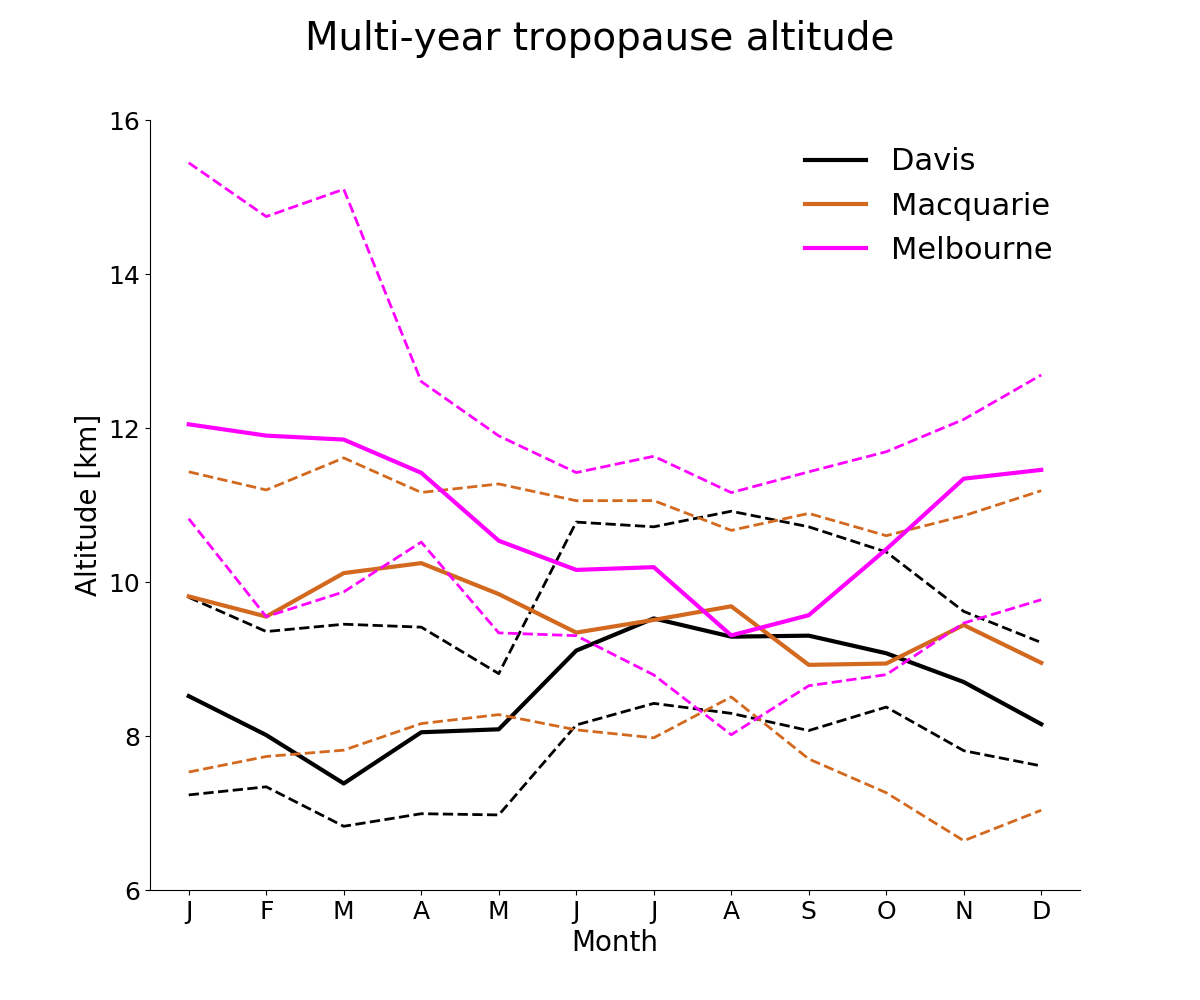
\includegraphics[width=0.8\columnwidth]{figures/tpheights}
      \caption{Multi-year monthly median tropopause altitude (minimum of lapse rate and ozone defined tropopause) determined from ozonesondes measurements at Melbourne (2004-2013), Macquarie (2004-2013) and Davis (2006-2013) (solid lines).
      Vertical shading shows the 10th to the 90th percentile of tropopauses for each site.
      }
      \label{fig:seasonaltpheights}
    \end{center} \end{figure}

    Figure \ref{fig:seasonaltropozone} shows multi-year averaged ozone mixing ratios measured by ozonesonde over the three stations.
    Over Melbourne, increased ozone extending down through the troposphere is apparent from December to March and September to November.
    The increased tropospheric ozone in these months are due to STTs (in summer), and possible fire smoke plume influence (in winter), discussed in more detail below.
    Over Davis and Macquarie Island, the tropospheric ozone is higher between March and October, although the seasonal differences are small compared to those at Melbourne.
    This seasonality at the high latitude sites is driven by a decrease in photochemical destruction when the solar zenith angle is greater, causing light to have longer path length and reduced radiation (TODO: read and cite S. Oltmans antarctic papers - re Andrews comment).
    
    \begin{figure}[!htbp]
      %Figure created seasonal_tropozone function in examine stations - ported from IDL
      \begin{center}
      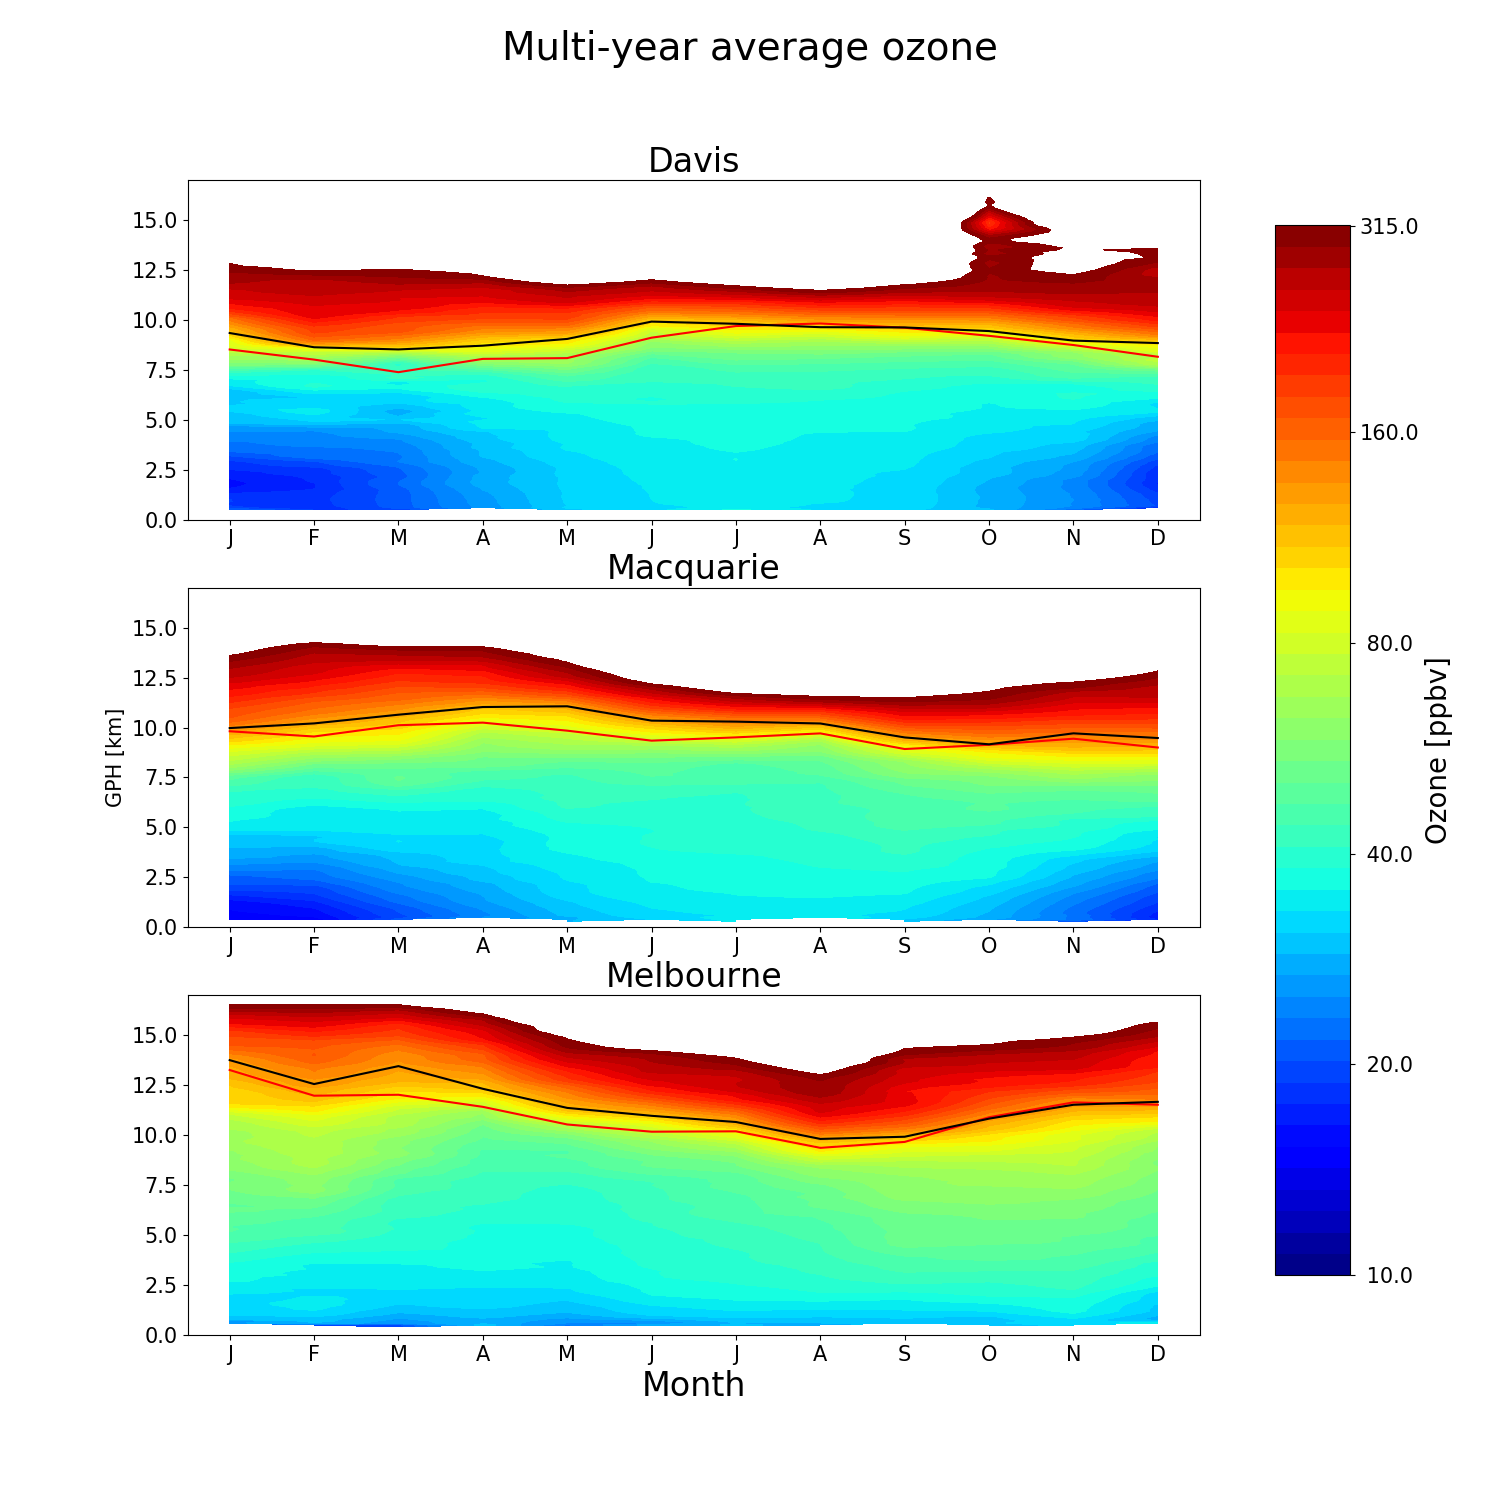
\includegraphics[width=0.95\columnwidth]{figures/seasonaltropozone}
      \caption{
      Multi-year mean seasonal cycle of ozone mixing ratio over Davis, Macquarie, and Melbourne measured by ozonesondes.
      Measurements were interpolated to every 100~m and then binned monthly.
      Black, red solid lines show median ozone and lapse-rate tropopause altitudes, defined as described in the text.
      }
      \label{fig:seasonaltropozone}
      \end{center}
    \end{figure}

  \subsection{Model description}
    \label{Section:GEOSChemDescription}
    GEOS-Chem is a global chemical transport model \citep{Bey2001}, which includes transport, emission, deposition, chemical production and destruction of ozone and 103 other trace gases throughout the troposphere along with stratospheric chemistry, including photolysis. 
    Stratosphere-troposphere coupling is calculated using the stratospheric unified chemistry extension (UCX) \citep{Eastham2014}, which includes a further 28 trace gases.
    For comparison to ozonesonde observations, we use GEOS-Chem version 10-011 (including UCX) run from 2005-2012, following a 1-year spin-up for 2004.
    Transport is driven by assimilated meteorological fields from the Goddard Earth Observing System (GEOS-5) maintained by the Global Modeling and Assimilation Office (GMAO) at NASA.
    Biogenic emissions of organic chemicals are determined by the Model of Emissions of Gases and Aerosols from Nature (MEGAN) version 2.1 extended by Guenther et al \citep{Guenther2012}.
    Anthropogenic emissions are given by the Emissions Database for Global Atmospheric Research (EDGAR) version 4.2.
  
    Our simulation was modified from the standard v10-01 to a fix a bug in the treatment of the Total Ozone Mapping Spectrometer (TOMS) satellite data used to calculate photolysis (see \citet{TomsFix2016}).
    The simulation uses 2$^{\circ}$ latitude by 2.5$^{\circ}$ longitude horizontal resolution, with 72 vertical levels from the surface to 0.1~hPa.
    The profile stored at each site is the average within the grid boxes which contain the site.
    For each site, a vertical profile of ozone is stored every 6 hours, based on standard UTC+0 time.
    This means that the GEOS-Chem profiles which match ozonesonde release hours are local times of 7AM, 11AM, and 11AM for Davis, Macquarie, and Melbourne respectively.
    
    
  \subsection{Characterisation of STT events and associated fluxes}
    \label{Section:CharacterisationOfSTTs}
    
    We characterise STT events using the ozonesonde vertical profiles to identify tropospheric ozone volume mixing ratio enhancements above a local background (in moles per billion moles of dry air, or ppb).
    Calculation of ozone transport is performed after converting the profile to molecules cm$^{-3}$.
    The process is illustrated in Figure~\ref{fig:filterEG} for an example ozone profile.
    
    \begin{figure}[!htbp]
      % Figure created in getevents.pro, edited in inkscape
      \begin{center}
      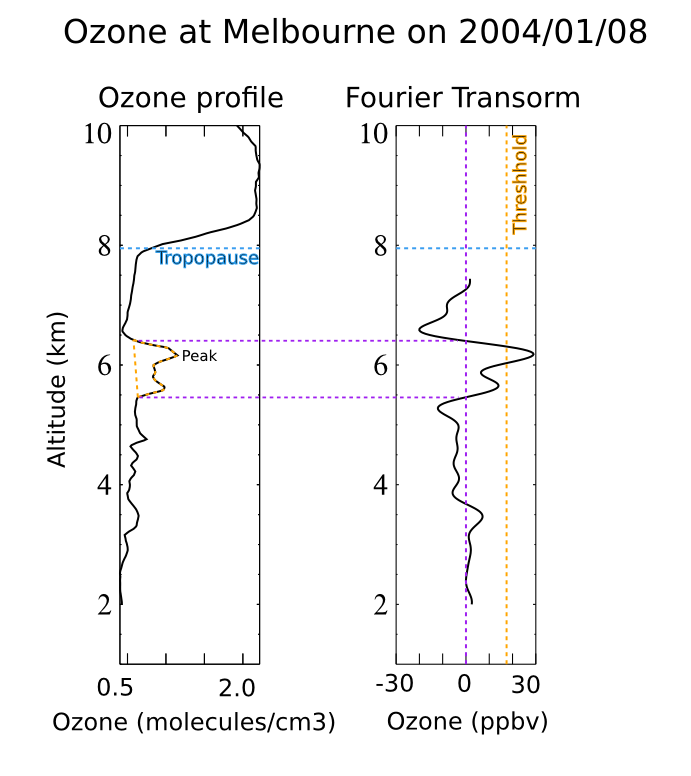
\includegraphics[width=0.8\columnwidth]{figures/filtereg.png}
      \caption{ An example of the STT identification and flux estimation methods used in this work. 
	The left panel shows an ozone mixing ratio profile from Melbourne on the 8th of January 2004 from 2km to the tropopause (dashed horizontal line).
	The right panel shows the perturbation profile created from bandpass filtering of the mixing ratio profile. The STT occurrence threshold calculated from the 99th percentile of filtered ozone perturbations is shown with the orange dashed line, and the technique for determining the vertical extent of the event is shown with the purple dashed lines (see details in text).
	The ozone flux associated with the STT event is calculated using the area outlined with the orange dashed line in the left panel.
      }
      \label{fig:filterEG}
      \end{center}
    \end{figure}
    
    First, the ozone vertical profiles are linearly interpolated to a regular grid with 20~m resolution from the surface to 14~km altitude. 
    The interpolated profiles are then bandpass filtered using a Fourier transform to retain perturbations with vertical scales between 0.5~km and 5~km (removing low and high frequency perturbations).
    In what follows, these filtered vertical profiles are referred to as perturbation profiles.
    The choice of band limits was set empirically. 
    For an event to qualify as STT, a clear increase above the background ozone level is needed, and we find that a vertical limit of $\sim 5$~km removes seasonal-scale effects.
    The 0.5~km scale limit is set in order to remove any spikes of ozone which could be considered noise.
    We next use all the perturbation profiles at each site to calculate the 99th percentile perturbation value for the site.
    This is considered our threshold for tropospheric ozone perturbations, and perturbations above this threshold in individual ozonesondes are classified as STT events.
    
    STTs which occur at altitudes below 4~km are removed in order to avoid surface pollution events
    Those occurring within 0.5~km of the tropopause are also removed in order to avoid spurious false positives induced by the sharp transition to stratospheric air.
    
    Finally, we define the ozone peak as the altitude where the OMR is greatest within the lowest range of altitudes where the perturbation profile exceeds the percentile-based threshold.
    If the perturbation profile drops below zero between the ozone peak and the tropopause, the STT event is confirmed. 
    Alternatively, if the OMR between the ozone peak and the tropopause drops below 80~ppb and is at least 20~ppb lower than the OMR at the ozone peak, the STT event is also confirmed. 
    Otherwise the profile is rejected as a non-event.
    This final step removes near-tropopause anomalies for which there is no evidence of detachment from the stratosphere.

    We estimate the ozone flux into the troposphere associated with each event by integrating the ozone concentration enhancement vertically over the altitude range for which an STT event is identified (i.e. the range surrounding the ozone peak over which the perturbation profile is greater than zero).
    This estimate is conservative because it does not take into any secondary ozone enhancements that may have been caused by the STT, and also ignores any heightened ozone background levels which may be due to synoptic-scale stratospheric mixing into the troposphere.
    
    \citet{Tang2010} define one possible method for detecting STT events from ozonesonde measurements. 
    Their definition is based on subjective analysis of sondes released from 20 stations in the latitudinal range from 35$^\circ$S to 40$^\circ$N.
    In their work, a tropopause fold has occurred if, starting from 5~km altitude, the ozone level exceeds 80~ppb and then within 3~km decreases by 20~ppb or more to a value less than 120~ppb.

  \subsection{Biomass burning influenced events}
  \label{Section:BiomassBurning}
    The STT detection algorithm described in Section \ref{Section:CharacterisationOfSTTs} assumes all mid-upper troposphere ozone perturbations above the 99th percentile are caused by stratospheric intrusions. 
    In some cases, however, these perturbations may in fact reflect ozone production in lofted smoke plumes.
    Biomass burning in southern Africa and South America has previously been shown to have a major influence on atmospheric composition in the vicinity of our measurement sites \citep{Gloudemans2006, Edwards2006}, particularly from July to December \citep{Pak2003}.
    On occasion, Australian and Indonesian fires can also reach the mid-high southern latitudes, which is seen when examining the carbon monoxide (CO) from the AIRS (Atmospheric Infrared Sounder) instrument on board the Aqua satellite \citep{AIRS3STD}.
    
    %Ozone precursors include nitrogen oxides ($NO_x = NO + NO_2$) and non methane volatile organic compounds (NMVOCs). % too basic for here..
    Large biomass burning events emit substantial quantities of ozone precursors, some of which are capable of being transported long distances and driving ozone production far from the fire source \citep{Jaffe_2012}.
    Ozone production from biomass burning is complex and affected by photochemistry, fuel nitrogen load, and time since emission. 
    While ozone production occurs in some biomass burning plumes, this is not always the case; therefore ozone perturbations detected during transported smoke events may or may not be caused by the plume.
    We therefore flag all detected STT events found near smoke plumes but do not exclude them from our final dataset.
    
    %Biomass burning influence in the Southern Hemisphere comes mostly from Southern Africa and South America, however Australian fires from the midlatitudes, and Indonesian fires can also influence the ozonesonde release sites.
    %Transported biomass burning plumes influence the southern mid-latitudes generally between July and December \citep{Pak2003}.
    
    Possible biomass burning influence is identified using satellite observations of CO from the AIRS instrument.
    CO is emitted during incomplete combustion and is an effective tracer of long-range transport due to its long lifetime.
    In the Southern Hemisphere, biomass burning is the primary source of CO, making CO a good proxy for fire plumes (eg: \citet{Edwards2003,Sinha2004,Edwards2006,Mari2008}).(TODO: split citations to their most appropriate sentences)
    We use data from the AIRS (Atmospheric Infrared Sounder) instrument on board the Aqua satellite \citep{AIRS3STD}.
    To identify possible biomass burning influence, we visually inspected AIRS vertical columns CO in the vicinity of our three measurement sites for all dates with detected STT events.
    We diagnose smoke plumes as areas with elevated CO columns ($\sim 2 \times 10^{18}$ molecules cm$^{-2}$ or higher), and flag any sonde-detected STT event that occurs near a smoke plume.

    Figure \ref{fig:excludedeg} contrasts two days with and without signs of biomass burning influence near the Melbourne site (purple circle).
    17 October 2007 (top) shows a day where elevated CO suggests the site may have been influenced by long-range transport from African and/or South American biomass burning.
    In contrast, on 3 February 2006 (bottom) CO columns across the Southern Hemisphere show no influence from biomass burning.
    We screened all days with detected STT events except one event during which there were no available AIRS data (January 2010), and found that biomass burning may have influenced 21\% of events over Melbourne and 17\% of events over Macquarie island.
    These events are flagged in the following sections, and are not used in our calculation of total STT flux.
    All of the flagged events except for one (in January at Macquarie Island) occur within the Southern Hemisphere burning season (July to December).% burning season cite? \citep{Pak2003}.
    No events at Davis were influenced by smoke transport.
    
    \begin{figure}[!htbp]
      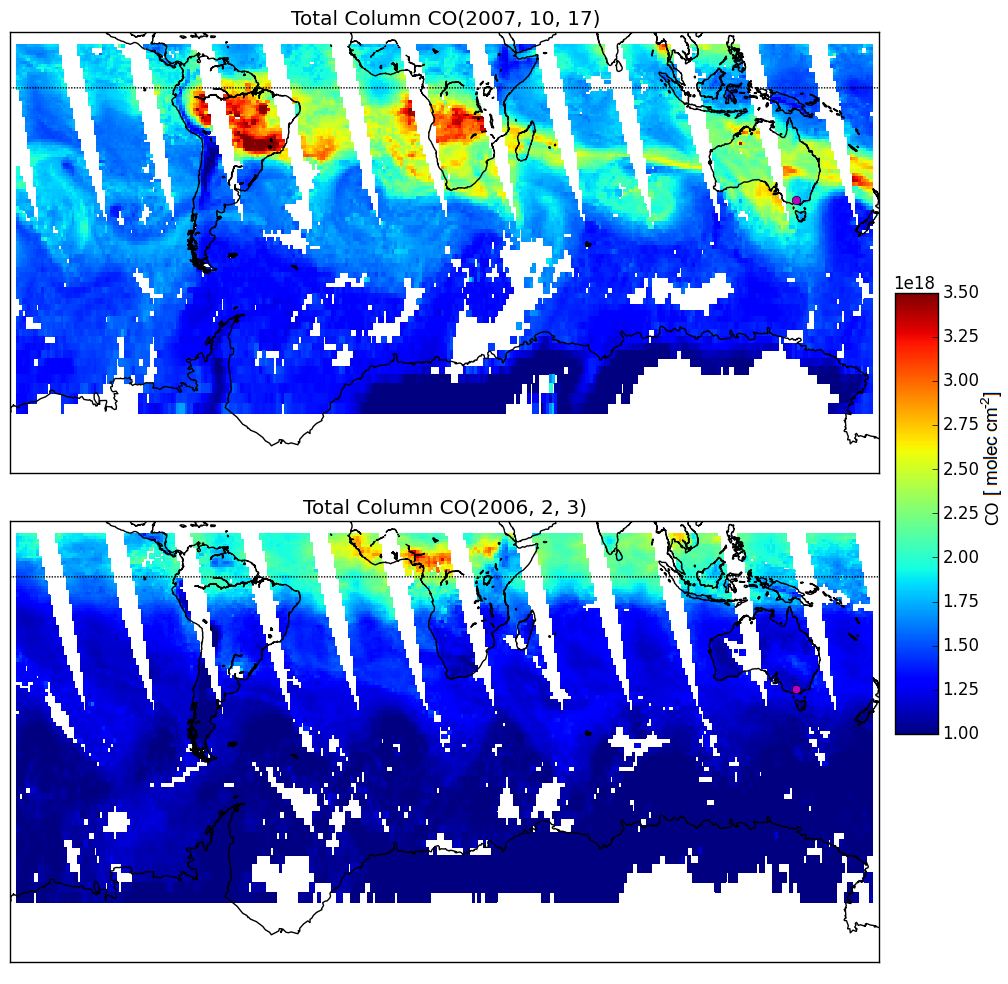
\includegraphics[width=\textwidth]{figures/AIRS_compare.png}
      \caption{ Example detection of biomass burning influence using AIRS total column CO. 
	The top panel (17 October 2007) shows a day when ozone above Melbourne (purple dot) could have been caused by a transported biomass burning plume, and so was flagged in subsequent analysis.
	The bottom panel (3 February 2006) shows a day when Melbourne ozone was not influenced by transported smoke.}
      \label{fig:excludedeg}
    \end{figure}
    
  \subsection{Sensitivities and limitations}
    Our method uses several subjectively defined quantities in the process of STT event detection.
    Here we briefly discuss these and the sensitivity to each.
    Using the algorithm discussed in section \ref{Section:CharacterisationOfSTTs}, we detect 45 events at Davis, 47 (+8 fire influenced) events at Macquarie Island, and 72(+14 fire influenced) events at Melbourne.
    
    The cut-off threshold (defined separately for each site) is determined from the 99th percentile of the ozone perturbations between 2~km and 1~km below the tropopause.
    We use the 99th percentile because at this point the filter locates clear events with no obvious false positives.
    Event detection is highly sensitive to this choice; for example, using the 98.5th percentile instead increased detected events by 24 at Melbourne (33\%), 19 at Macquarie Island (40\%), and 10 at Davis (22\%).
    This high sensitivity means that detection is also sensitive to the profile altitude bounds used in calculation of the percentiles, i.e. the 2~km altitude to 1~km below the tropopause range.
    The altitude range used to determine the 99th percentile is set from 2~km up to 1~km below the tropopause.
    This range removes any anomalous edge effects of the Fourier bandpass filter, as well as discounting the highly variable ozone concentration which occurs near the tropopause.
    Finally, ozone enhancements are only considered STT events if they occur above 4~km and within 500~m below the tropopause.
    This range removes possible ground pollution, as well as allowing event detection up to 500~m from the tropopause.
    Some events, including the storm-caused event examined in figure \ref{fig:Melbourne20050203} are within one kilometer of the tropopause. 
    
    The event detection was not as sensitive to the choice of Fourier bandpass scales; A widening of the allowed scales to the range 0.4-5.1 increased the detected events by 3 at Melbourne, 2 at Macquarie Island, and Davis lost two events (there are more detected events, but more being filtered out).
    
    Flux estimation over the southern ocean is based on the average GEOS-Chem tropospheric vertical column of HCHO over a particular latitude range.
    The range is from 35$^{\circ}$S to 75$^{\circ}$S, changing this latitude range by 5$^{\circ}$ in either direction at either end of the range changes the average simulated tropospheric ozone by -8 to 9\%.

  \subsection{Classifying synoptic conditions during STT events}
  \label{Section:WeatherClassifications}
    An investigation of the ERA-I synoptic weather during STT events above (at 500~hPa) Melbourne, Macquarie Island, and Davis are used to subjectively classify the events based on their likely cause.
    Typically during STT occurrence, the upper troposphere is not calm, with low pressure fronts or cut-offs nearby at coincident time.
    Similar characteristics are seen over Melbourne and Macquarie Island: i.e. a prevalence of frontal and low pressure activity during STT events.
    Over Davis the weather systems are harder to distinguish, and the stratospheric polar vortex may create ozone folds without other sources of upper tropospheric turbulence.

    We examine two case studies in detail to illustrate the synoptic-scale conditions in which STT events occur over Melbourne.
    Data from the European Center for Medium-range Weather Forecasts (ECMWF) Interim Reanalysis (ERA-I) \citep{Dee2011} product are used for synoptic-scale examination of weather patterns over our three sites on dates matching detected STT events.
    
    Figure \ref{fig:Melbourne20050203} (left) shows the ozonesonde profile above Melbourne on 3 of February 2005.
    The tropopause was between 400 and 500 hPa and ozone in the upper troposphere was anticorrelated with relative humidity, suggesting the ozone enhancements derived from dry stratospheric air. 
    An ozone intrusion into the troposphere at $\sim520$~hPa was identified by our detection algorithm.
    Figure \ref{fig:Melbourne20050203}(right) shows the concurrent synoptic weather system, a cut-off low pressure system that caused a large storm and lowered the local tropopause height for several days.
    These systems also increase turbulence near the tropopause, which can lead to increased transport events.
    %The wind circles around the low pressure system in a clockwise direction, typical geostrophic flows which are caused by pressure gradients and coriolis forces.
    The flux of stratospheric ozone into the troposphere associated with this event, calculated using the method shown in section \ref{Section:CharacterisationOfSTTs}, was at least $3.1 \times 10^{11}$ molecules cm$^{-3}$ , or 8\% of the tropospheric ozone column.

    \begin{figure}[!htbp]
    % these IMAGE CREATED BY show_profile.py, EDITTED IN INKSCAPE and then PINTA
      \begin{center}
      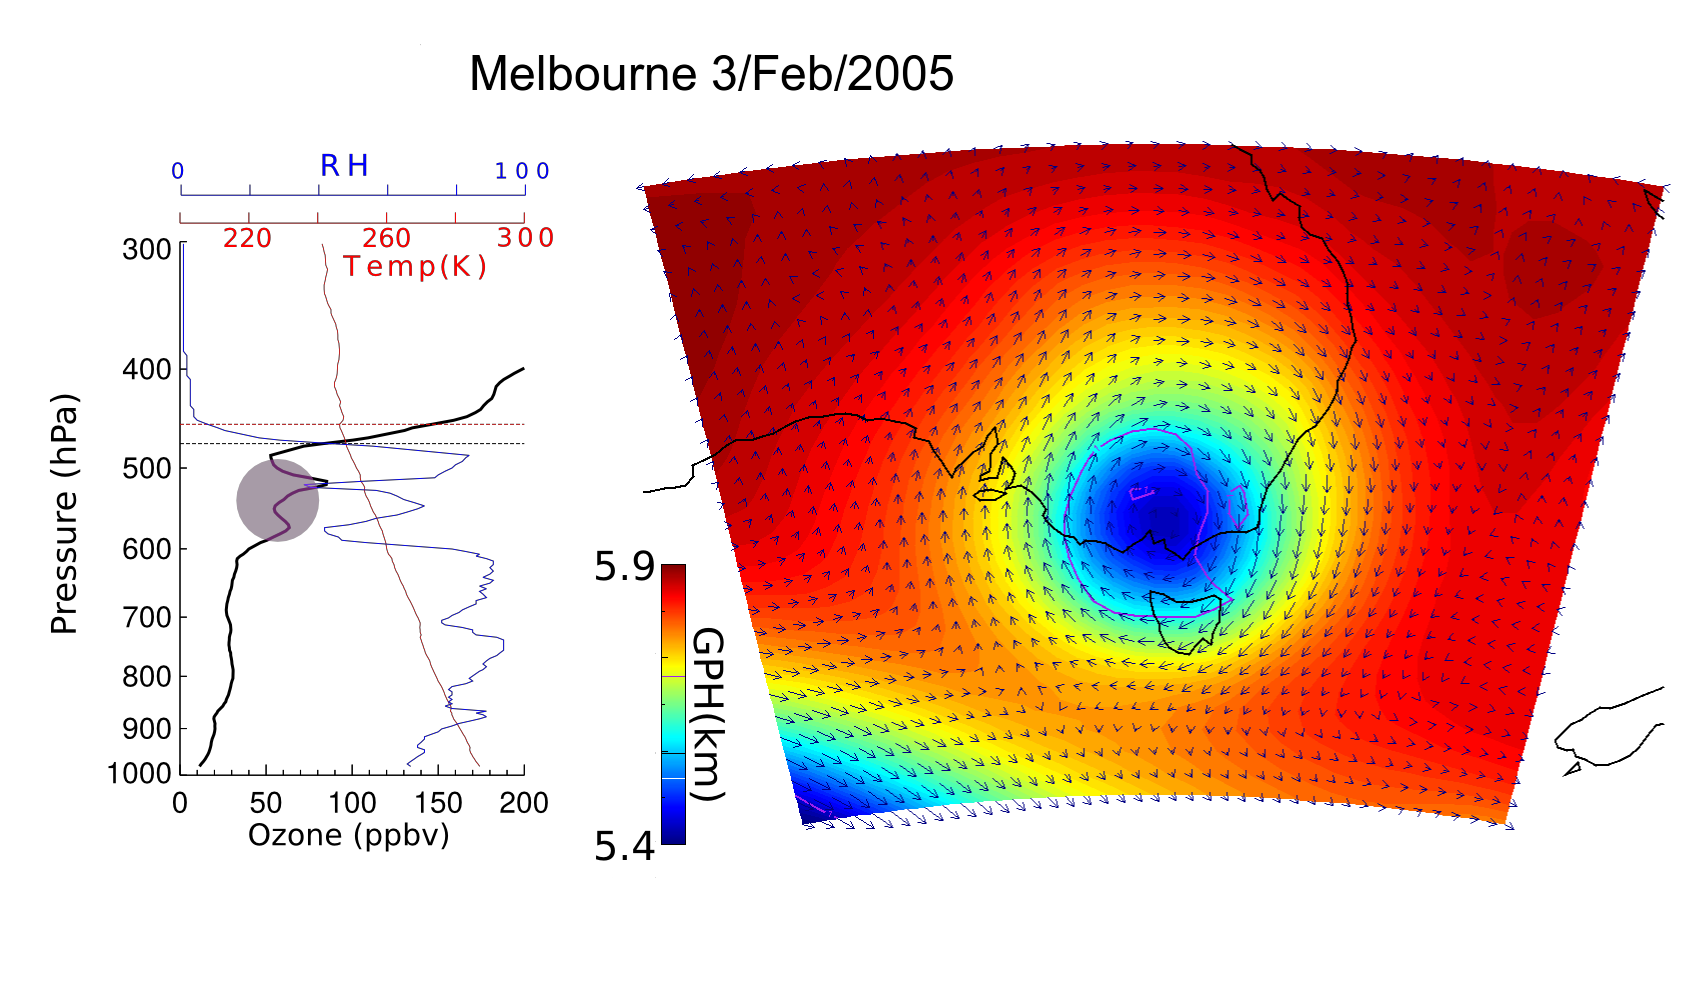
\includegraphics[width=1.0\columnwidth]{figures/Melbourne20050203.png}
      \caption{(Left) Vertical profile of ozone (black), relative humidity (blue), and temperature (red) measured by ozonesonde over Melbourne on 3 February 2005.
      The detected ozone STT event is highlighted in pink.
      Tropopause heights using both the ozone definition (black dashed line) and lapse rate definition (red dashed line) are also shown.
      (Right) Geopotential heights at 500 hPa from the ERA-Interim reanalysis, with wind vectors overplotted.
      Also shown are contours of potential vorticity units with 1 PVU in purple.}
      \label{fig:Melbourne20050203}
      \end{center}
    \end{figure}
    
    Figure \ref{fig:Melbourne20100113} (left) shows the vertical ozonesonde profile recorded on the 13th January 2010 over Melbourne.
    Figure \ref{fig:Melbourne20100113} (left) shows the ozonesonde profile over Melbourne on 13 January 2010.
    The tropopause was higher on this date (120-160 hPa).
    Using our algorithm, we detected an ozone intrusion centred around 200~hPa.
    As before, ozone anticorrelation with relative humidity provides further evidence that the elevated ozone was stratospheric in origin.
    In this profile, there was clear separation between the detected intrusion (highlighted in pink) and the ozone tropopause (black dashed line), which indicates that the sonde passed through regular tropospheric air after hitting a stratospheric intrusion but before reaching the tropopause.
    Figure \ref{fig:Melbourne20100113} (right) shows that this event was associated with a trough of low pressure (front) passing over southeastern Australia.
    This front traveled from west to east and caused a wave of lowered tropopause height. 
    Frontal passage is a known cause of STT as stratospheric air descends and streamers of ozone-rich air break off and mix into the troposphere \citep{Sprenger2003}.
    
    \begin{figure}[!htbp]
    % these IMAGE CREATED BY show_profile.py, EDITTED IN INKSCAPE
      \begin{center}
      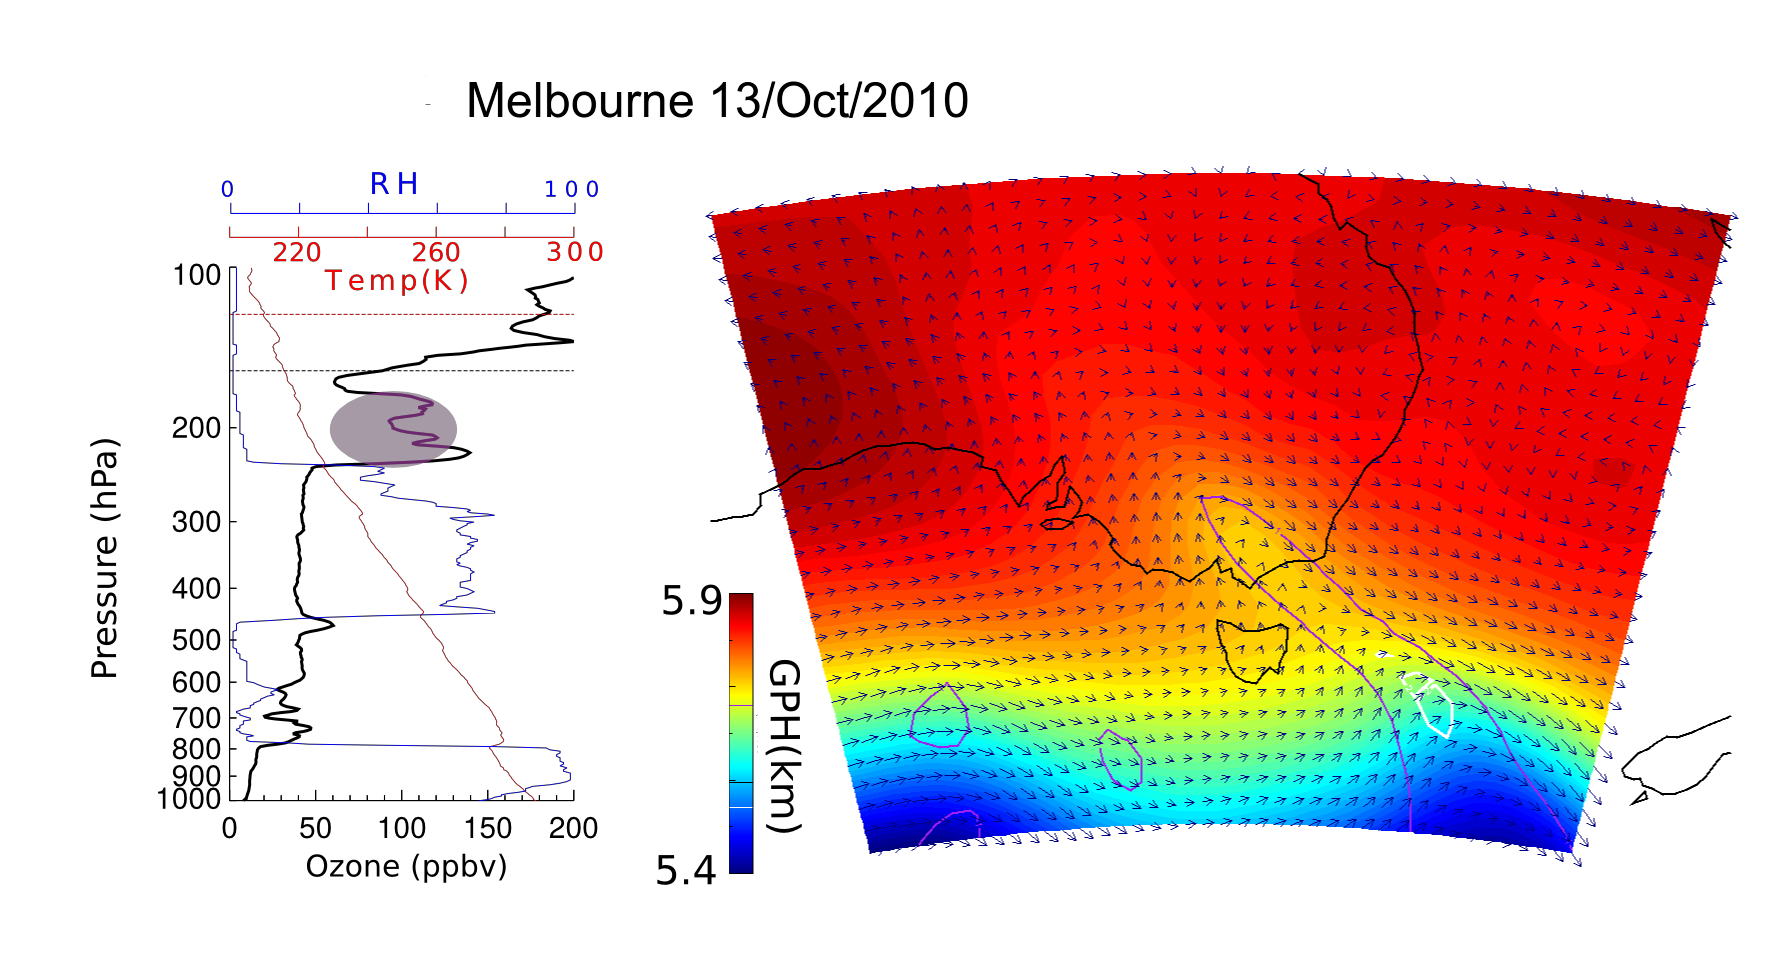
\includegraphics[width=1.0\columnwidth]{figures/Melbourne20100113.png}
      \caption{Same as Figure \ref{fig:Melbourne20050203} but for 13 January 2010.
	Also shown in this figure is the 2 PVU contour (white), often used to determine dynamical tropopause height.}
      \label{fig:Melbourne20100113}
      \end{center}
    \end{figure}

\section{STT event climatologies}
  
  re \ref{fig:SummarySeasonality} shows the seasonal cycles of STT events detected at Melbourne, Macquarie Island, and Davis. 
  STT events in Figures \ref{fig:SummarySeasonality}-\ref{fig:SummaryTPDepths} are coloured based on the meteorological classification described in Section \ref{Section:WeatherClassifications}, with events classified as either low pressure fronts (“frontal”, dark blue), cut-off low pressure systems (“cutoff”, teal), or indeterminate (“misc”, cyan).
  Events that may have been influenced by transported smoke plumes (Section \ref{Section:BiomassBurning}) are shown in red.
  (TODO: Event count, including types)
  
  There is an annual cycle in the frequency of STT events  (Fig. \ref{fig:SummarySeasonality}) with a summertime peak above Melbourne and Macquarie Island.
  This summertime peak is due to an increased prevalence of summer low-pressure storms and fronts, which increase turbulence and lower the tropopause \citep{Reutter2015}.
  For both Melbourne and Macquarie Island, the STT events which are unlikely to be fire-related occur mostly in summer during these low pressure synoptic systems.

  \begin{figure}[!htbp]
  % these IMAGE CREATED BY non_transport_summary.py, labels edited IN INKSCAPE
    \begin{center}
    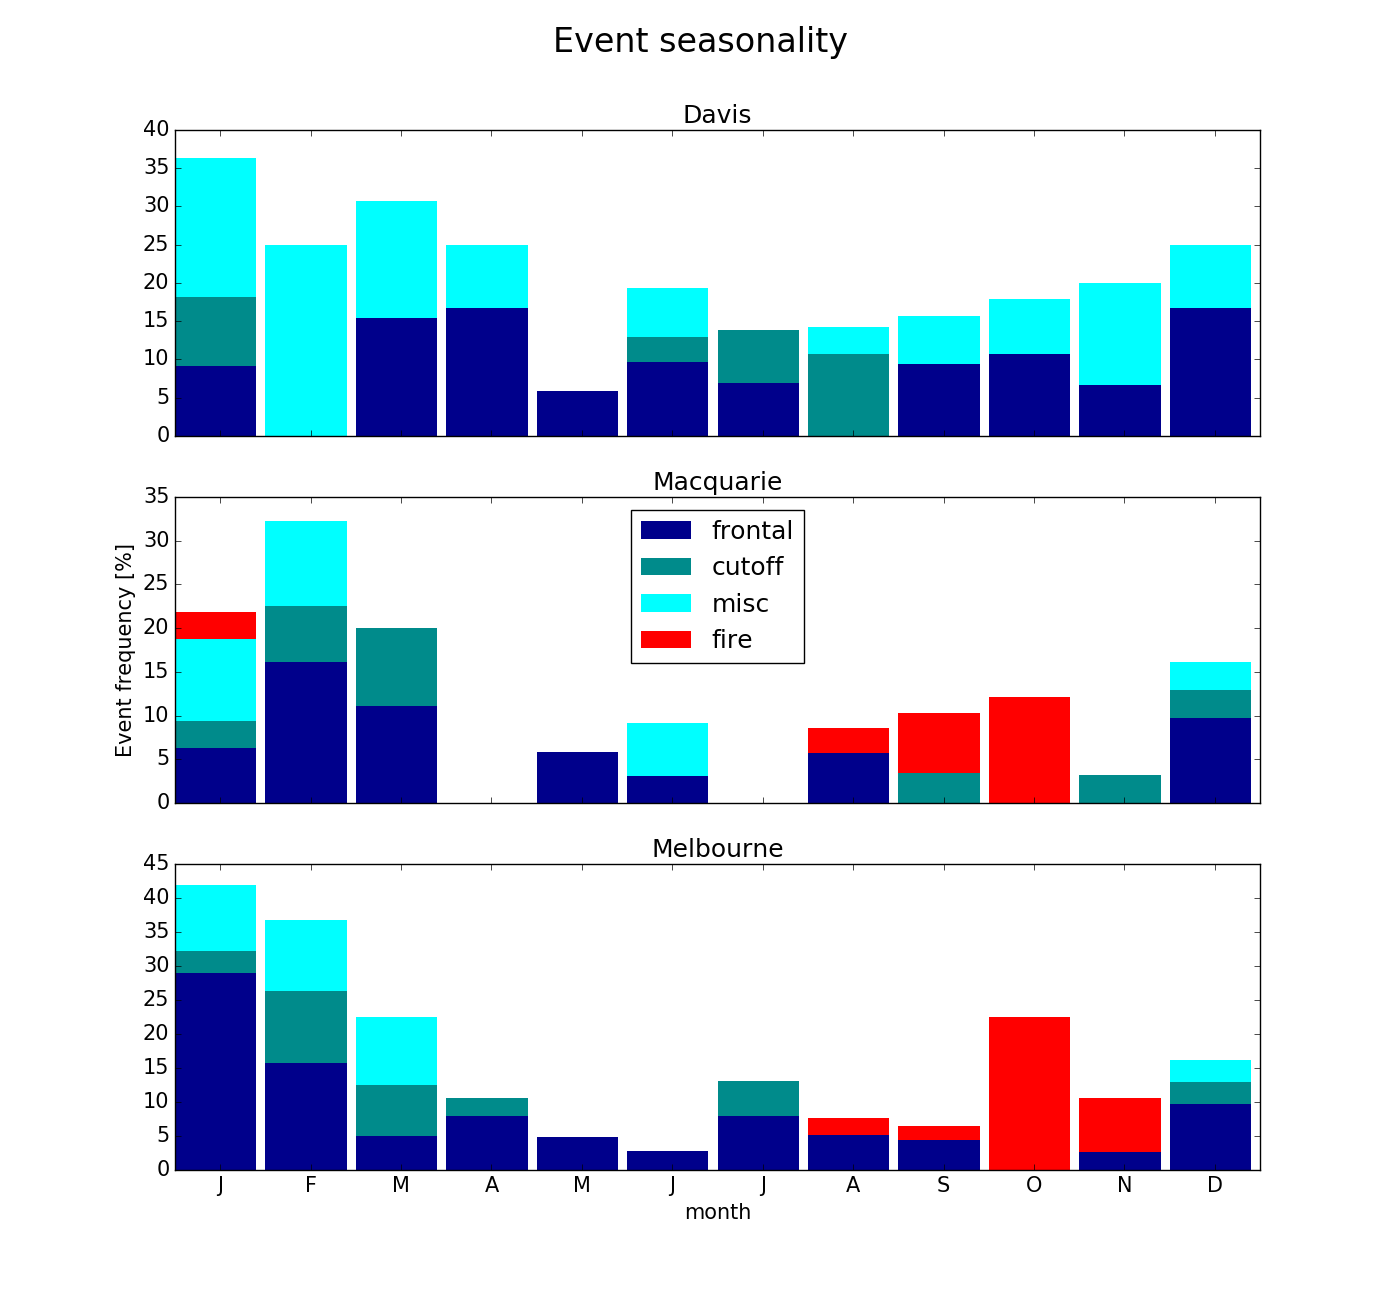
\includegraphics[width=1.0\columnwidth]{figures/summary_season.png}
    \caption{Seasonal cycle of STT events detected at Davis (top), Macquarie Island (middle), and Melbourne (bottom).
      Events are categorised by associated meteorological conditions as described in the text, with low pressure fronts (“frontal”) in dark blue, cut-off low pressure systems (“cutoff”) in teal, and indeterminate meteorology (“misc”) in cyan. 
      Events that may have been influenced by transported smoke plumes are shown in red (see text for details).}
    \label{fig:SummarySeasonality}
    \end{center}
  \end{figure}
  
  At Davis, the frequency of STT events is relatively constant throughout the year, with a slight increase during Antarctic winter.
  STT events associated with cut-off low pressure systems are more prevalent during winter, while STT events associated with frontal passage occur throughout the year. 
  The polar vortex and associated lowered tropopause may be partially responsible for the STTs detected in winter.
  We were unable to meteorologically classify most summertime events at Davis.

  The slightly increased winter time frequency of STT events at Davis may be attributable to the increased frequency of sonde releases from June to October (see Section \ref{Section:ozonesondes}).
  It is also possible that the sample of only 45 detected events over 10 years is too small to detect any seasonality.

  Figure \ref{fig:SummaryAltitudes} shows the altitudes of detected events, based on the altitude of peak (maximum) tropospheric ozone in the ozonesonde profile.
  STT event peaks most commonly occur at 6 -- 10~km above Melbourne and 6 -- 9~km at Davis but are distributed more evenly at Macquarie Island from ~4 -- 7.5 kilometres altitude.
  There is no clear relationship between meteorological conditions and event altitude.

  Figure \ref{fig:SummaryTPDepths} shows the distance from the tropopause of the peaks of detected events, based on the distance between the peak ozone peak associated with the detected STT event and the tropopause (using the lowest of the two tropopause definitions), as described in Section \ref{Section:ozonesondes}.
  The majority of STT events occur within 3~km of the tropopause at both Melbourne and Macquarie Island, and within 2~km of the tropopause at Davis. 
  Again, there is no clear relationships between meteorological conditions and event depth.

  \begin{figure}[!htbp]
    \begin{center}
    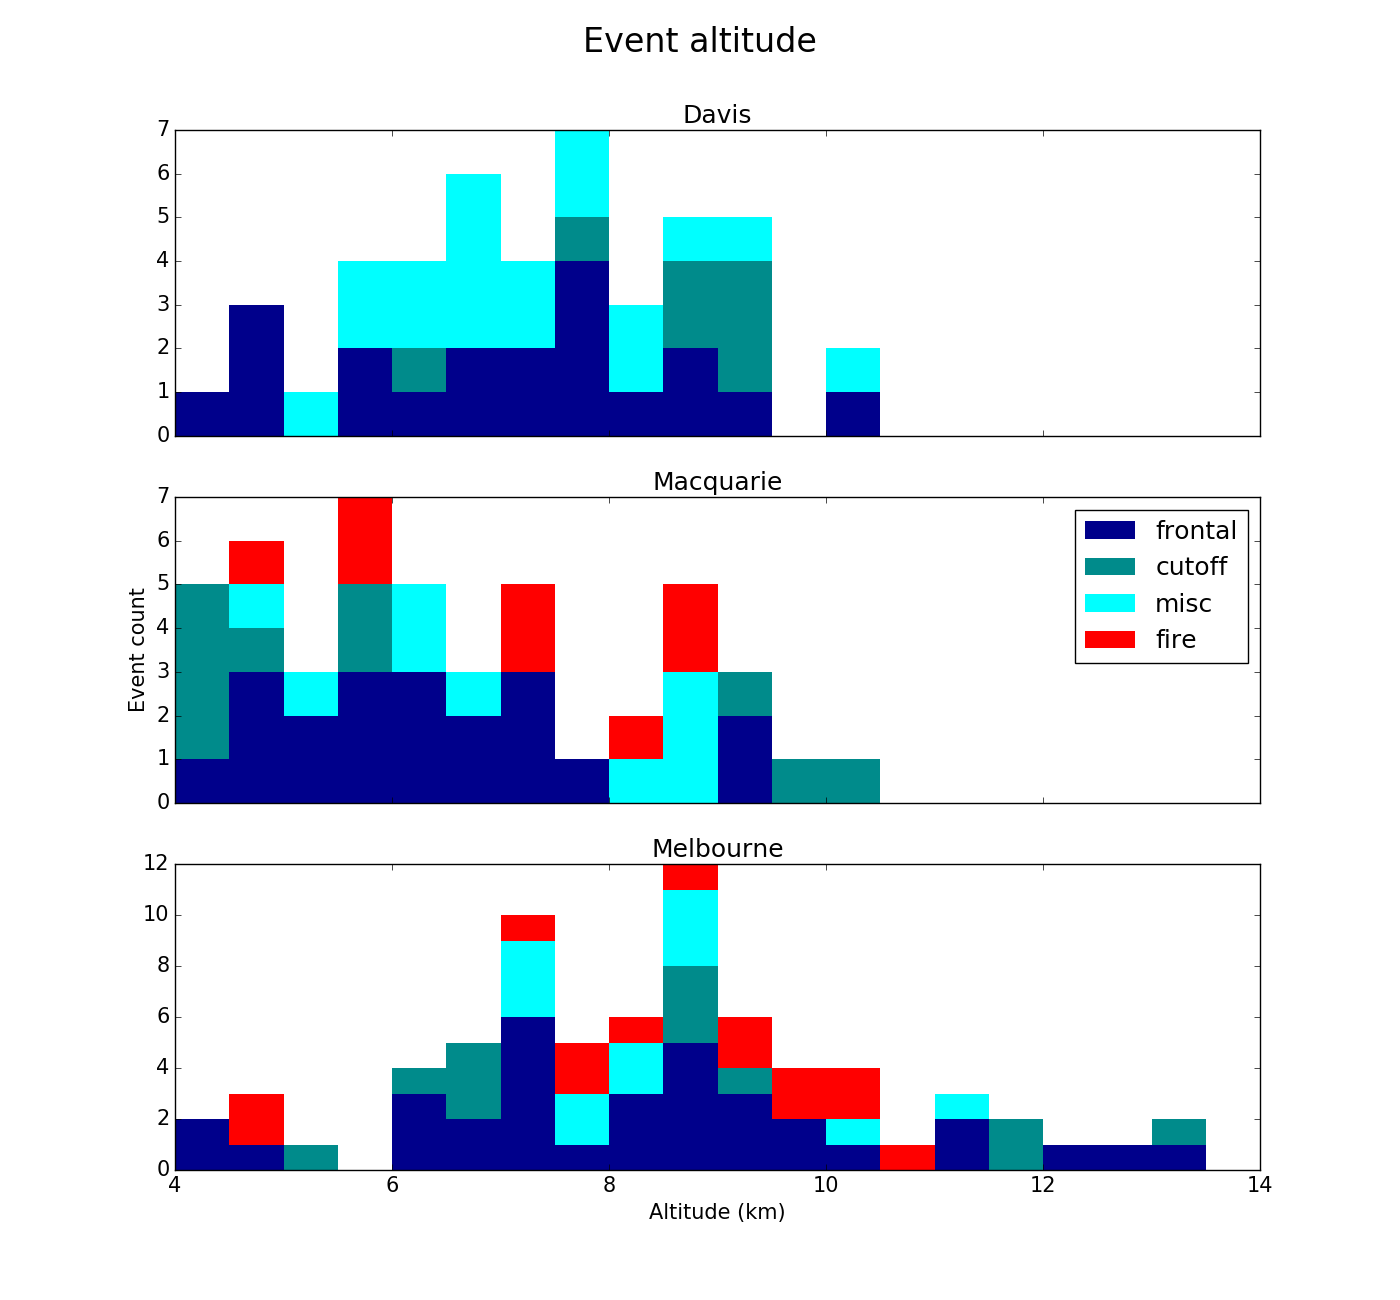
\includegraphics[width=0.99\columnwidth]{figures/summary_altitude.png}
    \caption{The distribution of STT event altitude at Davis (top), Macquarie Island (middle), and Melbourne (bottom), determined as described in the text.
    Events are coloured as described in Fig. \ref{fig:SummarySeasonality}.}
    \label{fig:SummaryAltitudes}
    \end{center}
  \end{figure}

  \begin{figure}[!htbp]
    \begin{center}
    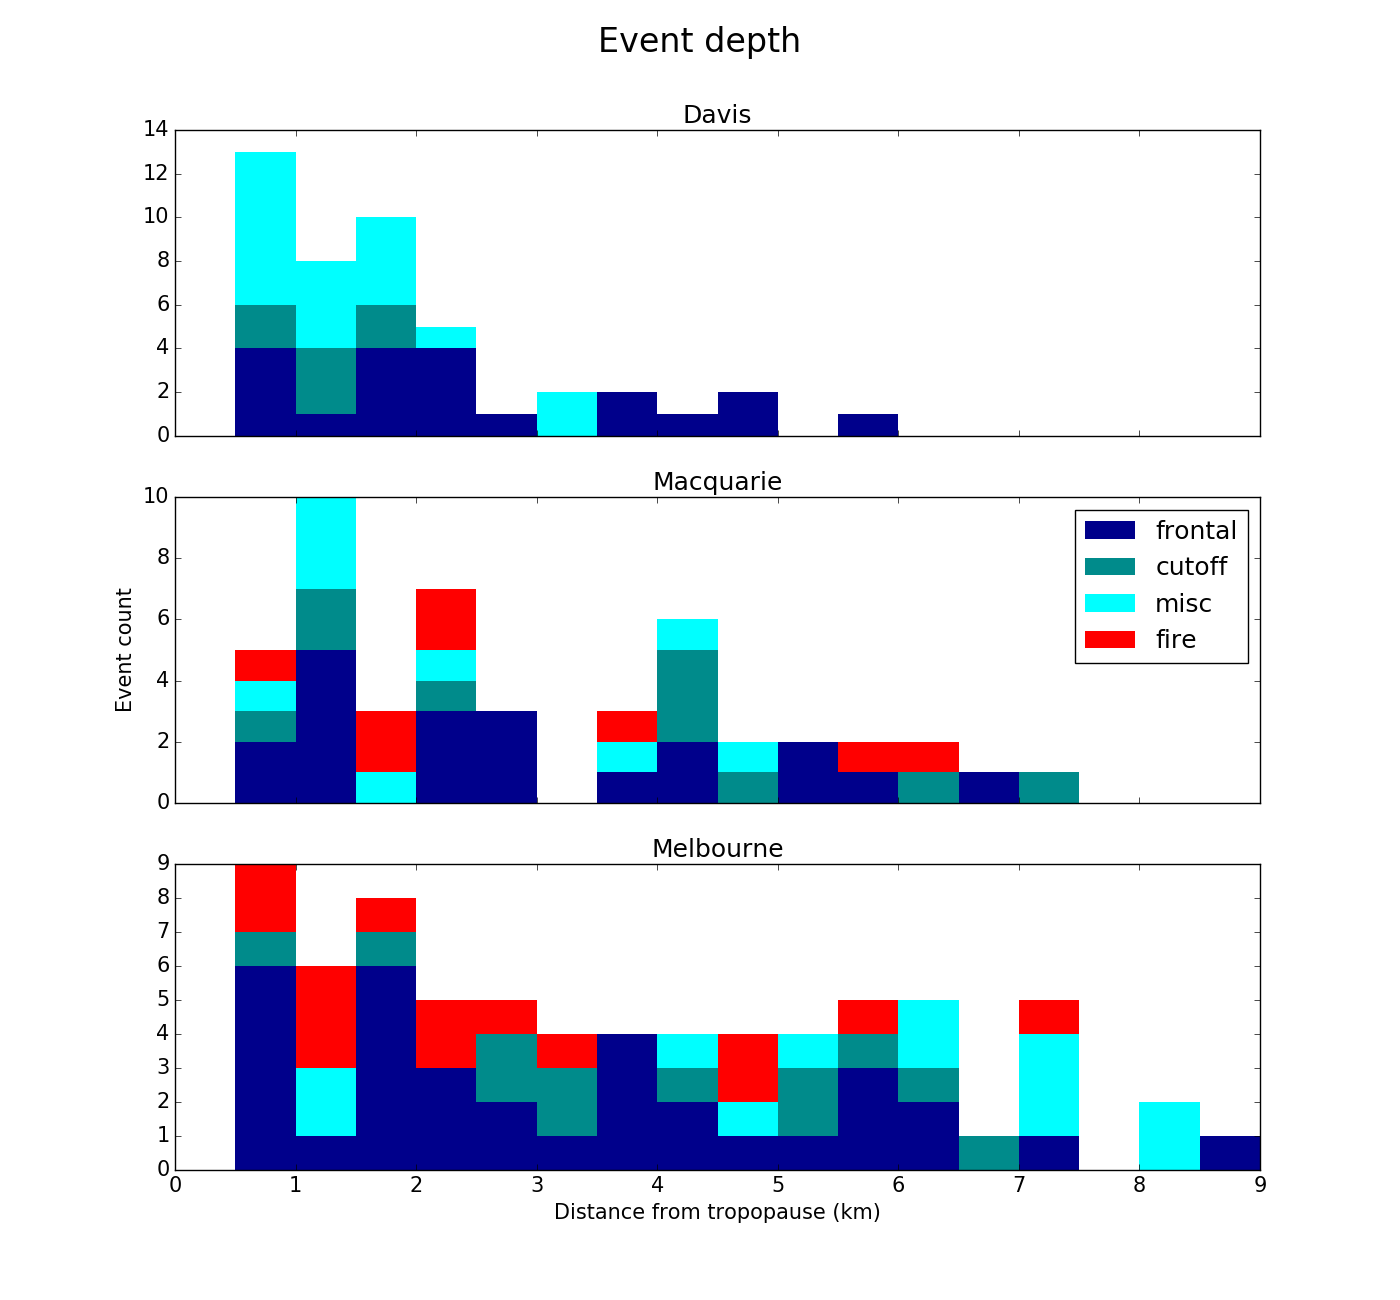
\includegraphics[width=0.99\columnwidth]{figures/summary_depth.png}
    \caption{The distribution of STT event distance from the tropopause at Davis (top), Macquarie Island (middle), and Melbourne (bottom), determined as described in the text.
    Events are coloured as described in Fig. \ref{fig:SummarySeasonality}.}
    \label{fig:SummaryTPDepths}
    \end{center}
  \end{figure}

\section{Comparison with GEOS-Chem}
  
  \begin{figure}[!htbp]
    % made in examine_stations.py in stations repository
    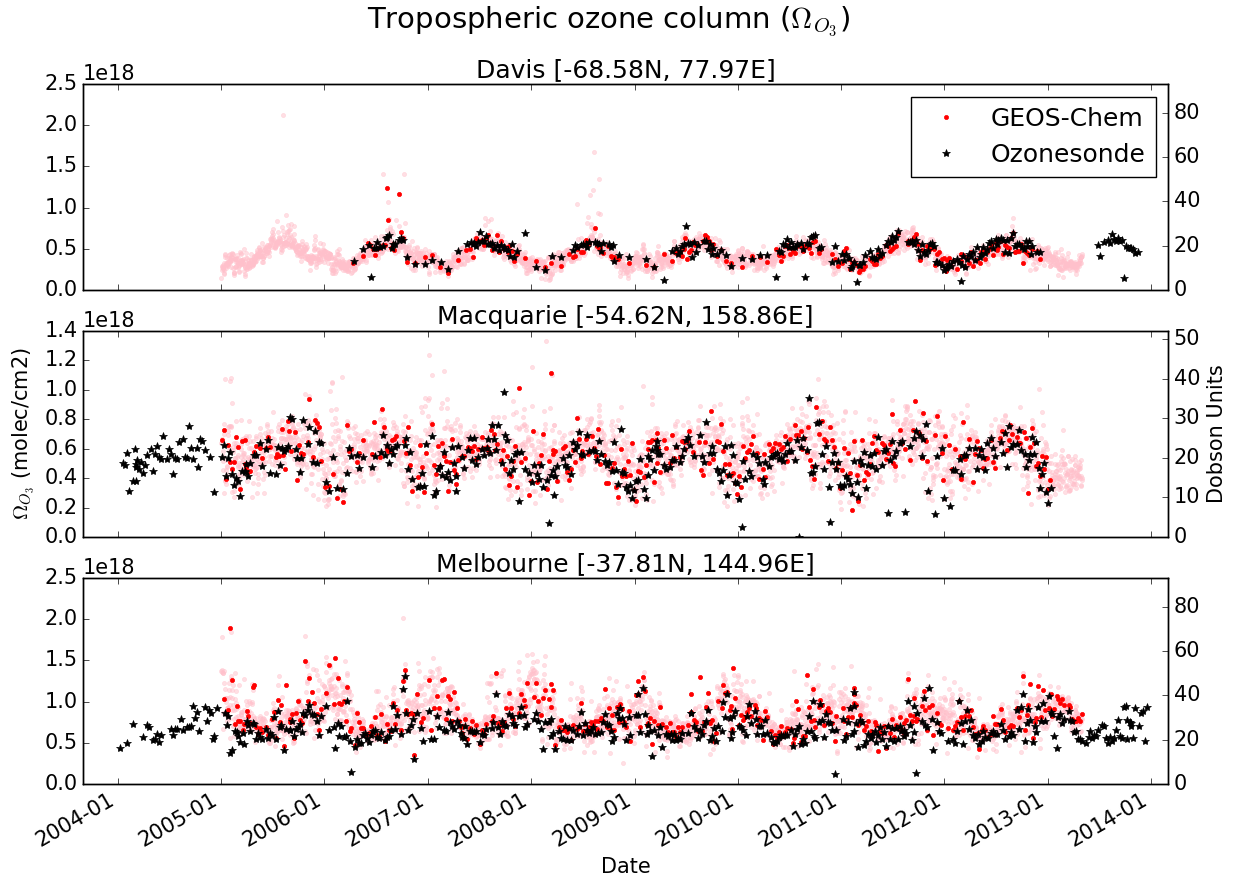
\includegraphics[width=\textwidth]{figures/StationSeries.png}
    \caption{Tropospheric ozone column ($\Omega_{O3}$, in molecules cm$^{-2}$) at daily resolution simulated by GEOS-Chem (grey dots) from January 1 2004 to April 31 2013.
    Simulated points which are on the same day as an ozonesonde are displayed in red.
    For each plot, the model has been sampled in the grid square containing the site.
    Columns calculated from ozonesondes are shown as black stars, each representing one measurement.}
    \label{fig:StationSeriesGEOSChem}
  \end{figure}
  
  Figure \ref{fig:StationSeriesGEOSChem} compares the time series of tropospheric ozone column ($\Omega_{O_3}$) in molecules cm$^{-2}$ simulated by GEOS-Chem (red dots) to the measured tropospheric ozone columns (black stars).
  Sonde tropospheric columns are calculated using the GPH and ozone partial pressure recorded by the ozonesondes, using (TODO: equation here.)
  The seasonal cycles are well correlated, with similar timing and magnitude (paired r$^2$ values of TODO: run script when model run finished). 
  In both observations and model, the maximum ozone column at Melbourne occurs in summer, with a minimum in winter, while Macquarie and Davis show the opposite seasonality.
  The model shows more day-to-day variability than the ozonesondes, although there are daily simulated values for the model while only weekly or less for the ozonesondes. (TODO: Verify this)
  
  \begin{figure}[!htbp]
    % Created in examine_stations.py
    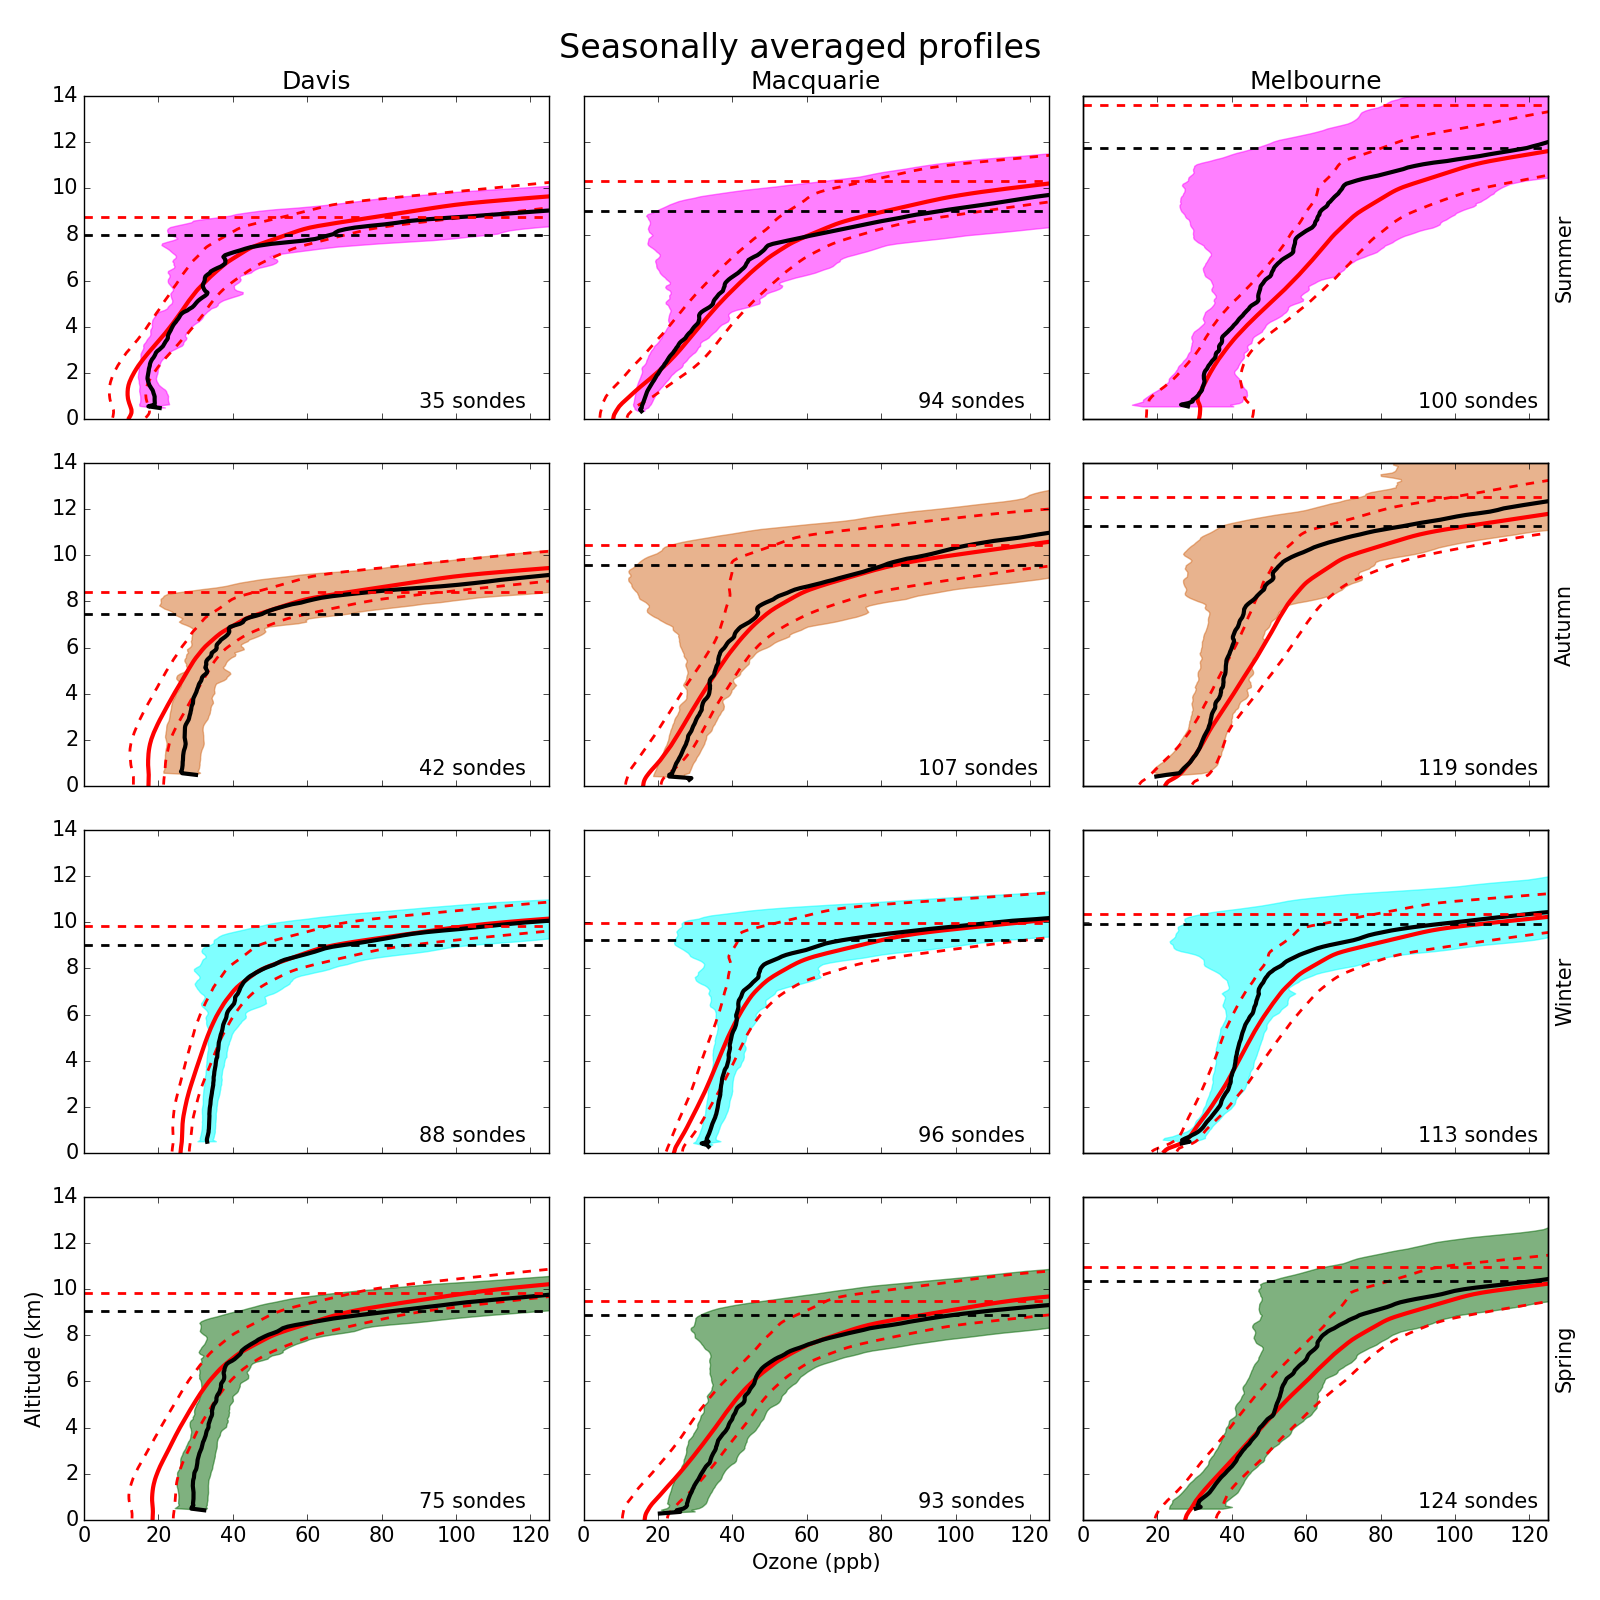
\includegraphics[width=\textwidth]{figures/seasonalprofiles00.png}
    \caption{Observed and simulated tropospheric ozone profiles over Davis, Macquarie, and Melbourne, averaged seasonally.
    Model means (2005-2013 average) is shown as red solid lines, with red dashed lines showing the 10th and 90th percentile.
    Ozonesonde means (over each season, for all years) are shown as black solid lines, with coloured shaded areas showing the 10th and 90th percentile.
    The horizontal dotted line shows the mean tropopause heights from the model (red) and the observations (black).}
    \label{fig:GEOSChemSeasonalProfiles}
  \end{figure}
  
  Figure \ref{fig:GEOSChemSeasonalProfiles} shows the observed and simulated ozone profiles at all sites, averaged seasonally.
  The model generally underestimates ozone at low altitudes (up to 6~km) at both Davis and Macquarie, although this bias is less pronounced during summer.
  Over Melbourne, ozone in the lower troposphere is well represented, but the model overestimates ozone from around 4~km to the tropopause.
  Also shown is the tropopause height simulated by the model (horizontal dashed red line), the mean of which is always higher than the observed average, although this difference is statistically insignificant.
  The effect of local pollution can be seen over Melbourne, mostly during the austral summer months (DJF), as the increased mean mixing ratios and enhanced variance near the surface.
  
  Although GEOS-Chem reasonably matches the ozonesonde tropospheric ozone column, it does not have the resolution required to capture STTs.
  Figure \ref{fig:event_profile_comparison} compares modeled (red) and observed (black) ozone profiles on three example days when STT events were detected using the ozonesondes. 
  The plot shows the profile with the closest (qualitative) match between model and observations; from left to right the profiles are from Davis yyyymmdd, Macquarie Island yyyymmdd, and Melbourne yyyymmdd. (TODO: update this plot)
  The vertical resolution from GEOS-Chem is too low to allow detection of STTs, with roughly 30 vertical levels up to the tropopause, while sondes have upwards of 100.
  
  \begin{figure}[!htbp]
    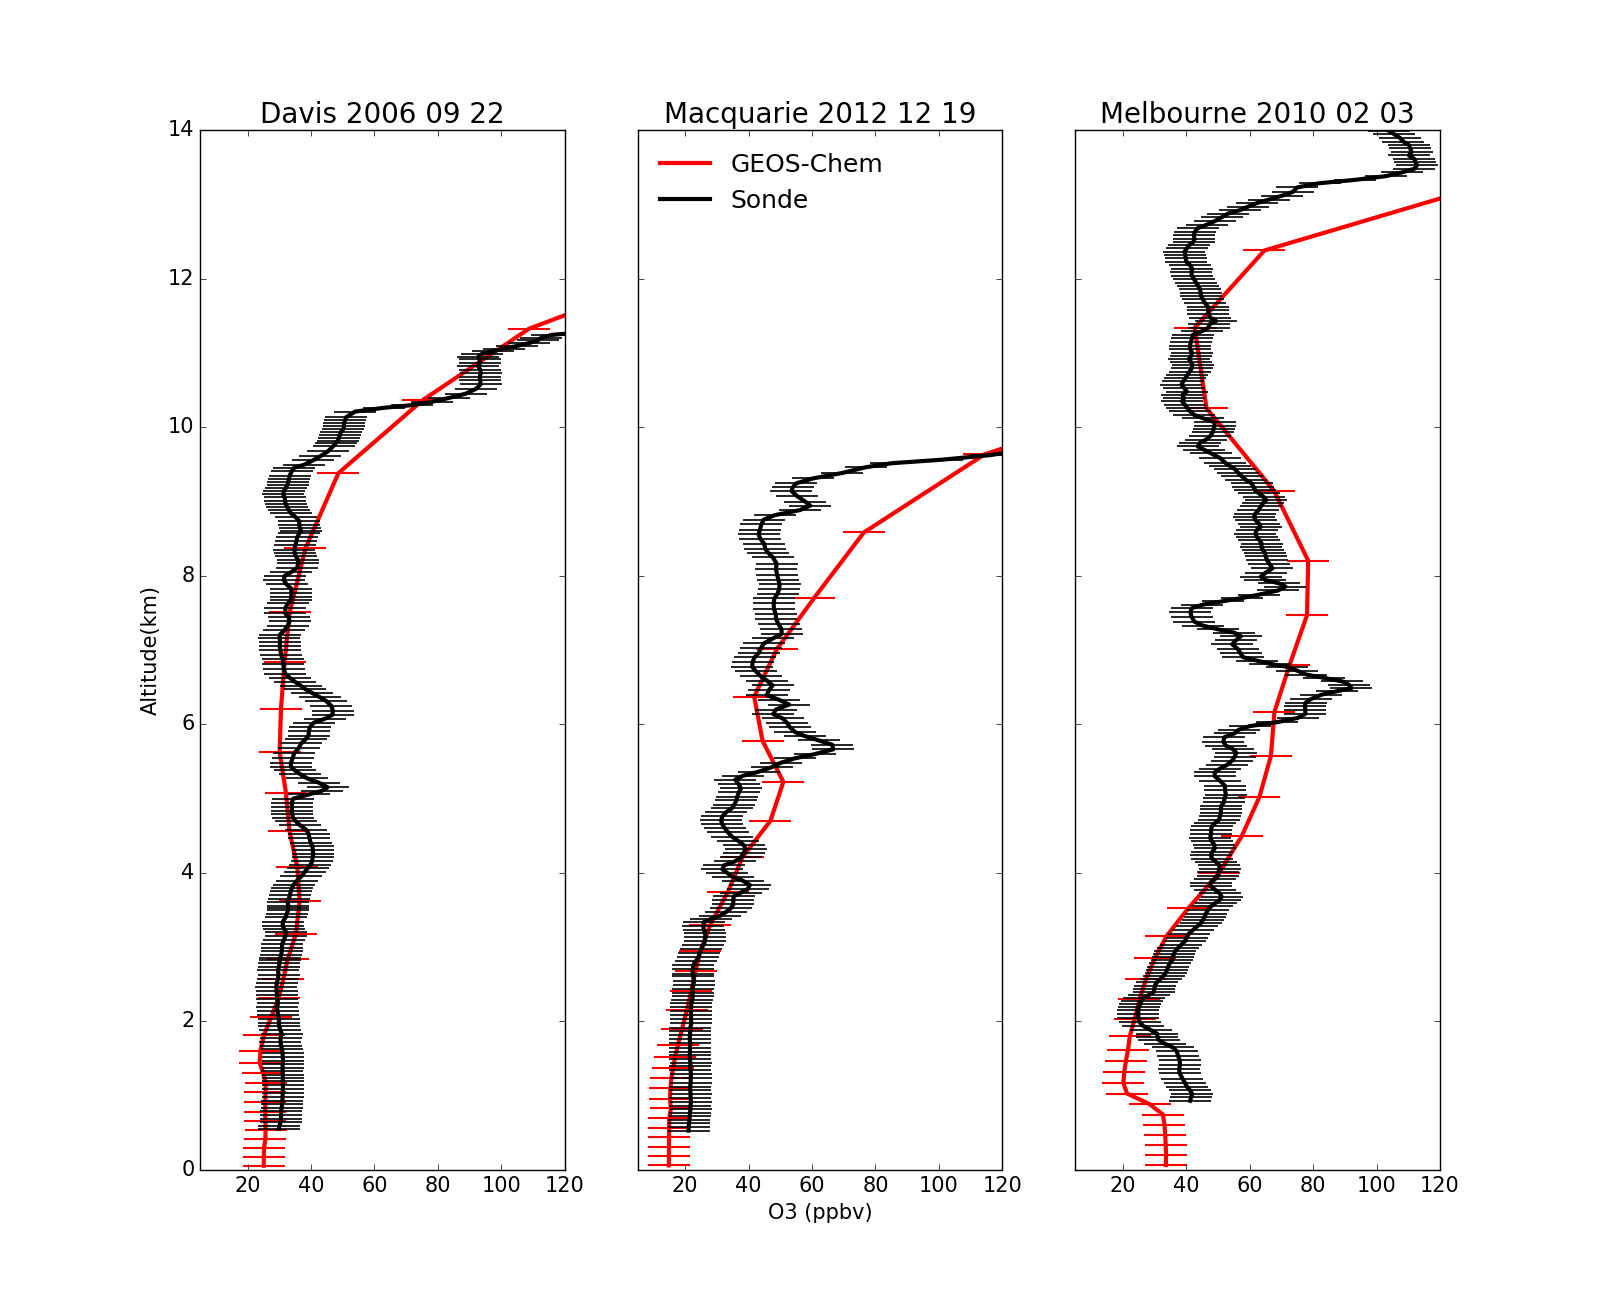
\includegraphics[width=\textwidth]{figures/event_profile_comparison.png}
    \caption{Example comparisons of ozone profiles from ozonesondes (black) and GEOS-Chem (red) from 		  three different dates during which STT events were detected from the measurements.
      The dates were picked based on subjective visual analysis. 
      The examples show the best match between model and observations for: (left) 19 May 2004 over Macquarie Island;  (middle) 15 January 2007 over Davis, and (right) 3 February 2005 over Melbourne.
      (TODO: update figure and caption dates, use best matches, show model pressure levels with Xs.}
    \label{fig:event_profile_comparison}
  \end{figure}
  
\section{Stratosphere-to-troposphere ozone flux from STT events}
  
  We quantify the mean stratosphere-to-troposphere ozone flux due to STTs at each site based on the integrated ozone amount associated with each STT event (see section \ref{Section:CharacterisationOfSTTs}).
  Events that may have been influenced by transported biomass burning are excluded from this calculation.
  This estimate is a conservative lower bound as our algorithm ignores secondary ozone peaks which may also be transported down from the stratosphere and also potential ozone enhancement due to the ozone intrusion which is outside the event positive perturbation range around the detected ozone peak.
  
  Figure \ref{fig:fluxsummary} shows the mean fraction of total tropospheric column ozone calculated from ozonesonde profiles at each site attributed to stratospheric ozone intrusions, averaged over days when an STT event occurred.
  At all sites, the mean fraction of tropospheric ozone attributed to STT events is 2--4\%. On individual days, this value can exceed 10\% at Macquarie and Melbourne.
  Figure \ref{fig:fluxsummaryabs} shows the STT-induced ozone flux in absolute terms.
  We find that the mean ozone flux associated with STT events is $1$ to $2 \times 10^{16}$~molecules/cm$^2$.
  Our flux estimates are relatively insensitive to our biomass burning filter: including smoke-influenced days changed the mean flux by less than 5\% relative to the absolute absolute values.
  
  \begin{figure}[!htbp]
  % Flux box and whisker plots from flux_summary.pro in OzoneWork(HPC) and edited in Inkscape
    \begin{center}
    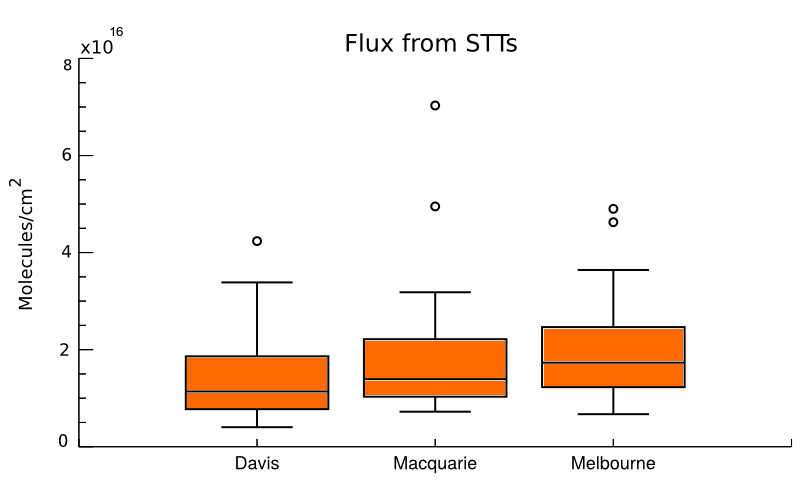
\includegraphics[width=0.8\columnwidth]{figures/flux_absolute.png}
    \caption{Tropospheric ozone attributed to STT, derived from ozonesonde measurements as described in the text.
      Box shows the interquartile range (IQR), with the centre line being the median, whiskers show the mininimum and maximum, circles show values which lie more than 1.5 IQR from the median.}
    \label{fig:fluxsummaryabs}
    \end{center}
  \end{figure}
  \begin{figure}[!htbp]
    \begin{center}
    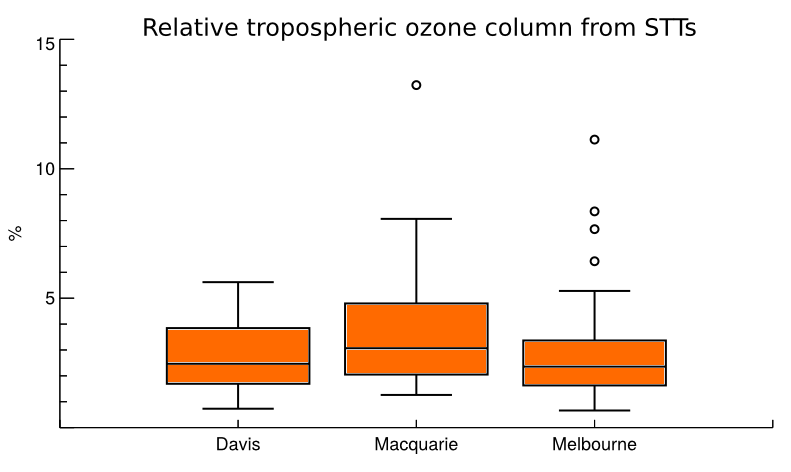
\includegraphics[width=0.8\columnwidth]{figures/flux_relative.png}
    \caption{Fraction of total tropospheric column ozone attributed to STT, derived from ozonesonde measurements as described in the text.}
    \label{fig:fluxsummary}
    \end{center}
  \end{figure}
  
  We use simulated tropospheric ozone columns from GEOS-Chem to extrapolate the sonde-based estimates to the entire Southern Ocean region. 
  To do so, we multiply the monthly likelihoods of STTs (fraction of sonde releases for which an STT event was detected, per month, `l') by the monthly mean tropospheric ozone column over the Southern Ocean (from the GEOS-Chem multi-year mean, $\Omega_{SO_{O_3}}$) and by the monthly mean fraction of the ozone column attributed to STT (`f') (as in Fig. \ref{fig:fluxsummary}, but separated by month).
  The monthly values of each term in this equation are shown in Figure \ref{fig:SOExtrapolation} (lower panel).
  The equation can be written simply: Flux$= \Omega_{SO_{O_3}} \times f \times l$.
  
  Figure \ref{fig:SOExtrapolation} shows the extrapolated monthly mean ozone flux from STT events over the Southern Ocean.
  We find that STT events may be responsible for at least $3.2 \times10^{16}$~molecules cm$^{-2}$ yr$^{-1}$, of the tropospheric ozone over the Southern Ocean, this is around 1.82~TG yr$^{-1}$ ozone.
  This is calculated using the surface area from GEOS-Chem over the southern ocean grid boxes along with the molecules cm$^{-2}$ per month calculations, along with ozone molar mass of 48~g mol$^{-1}$.
    
  \begin{figure}[!htbp]
    % Plot from examine_stations.py in stations repo
    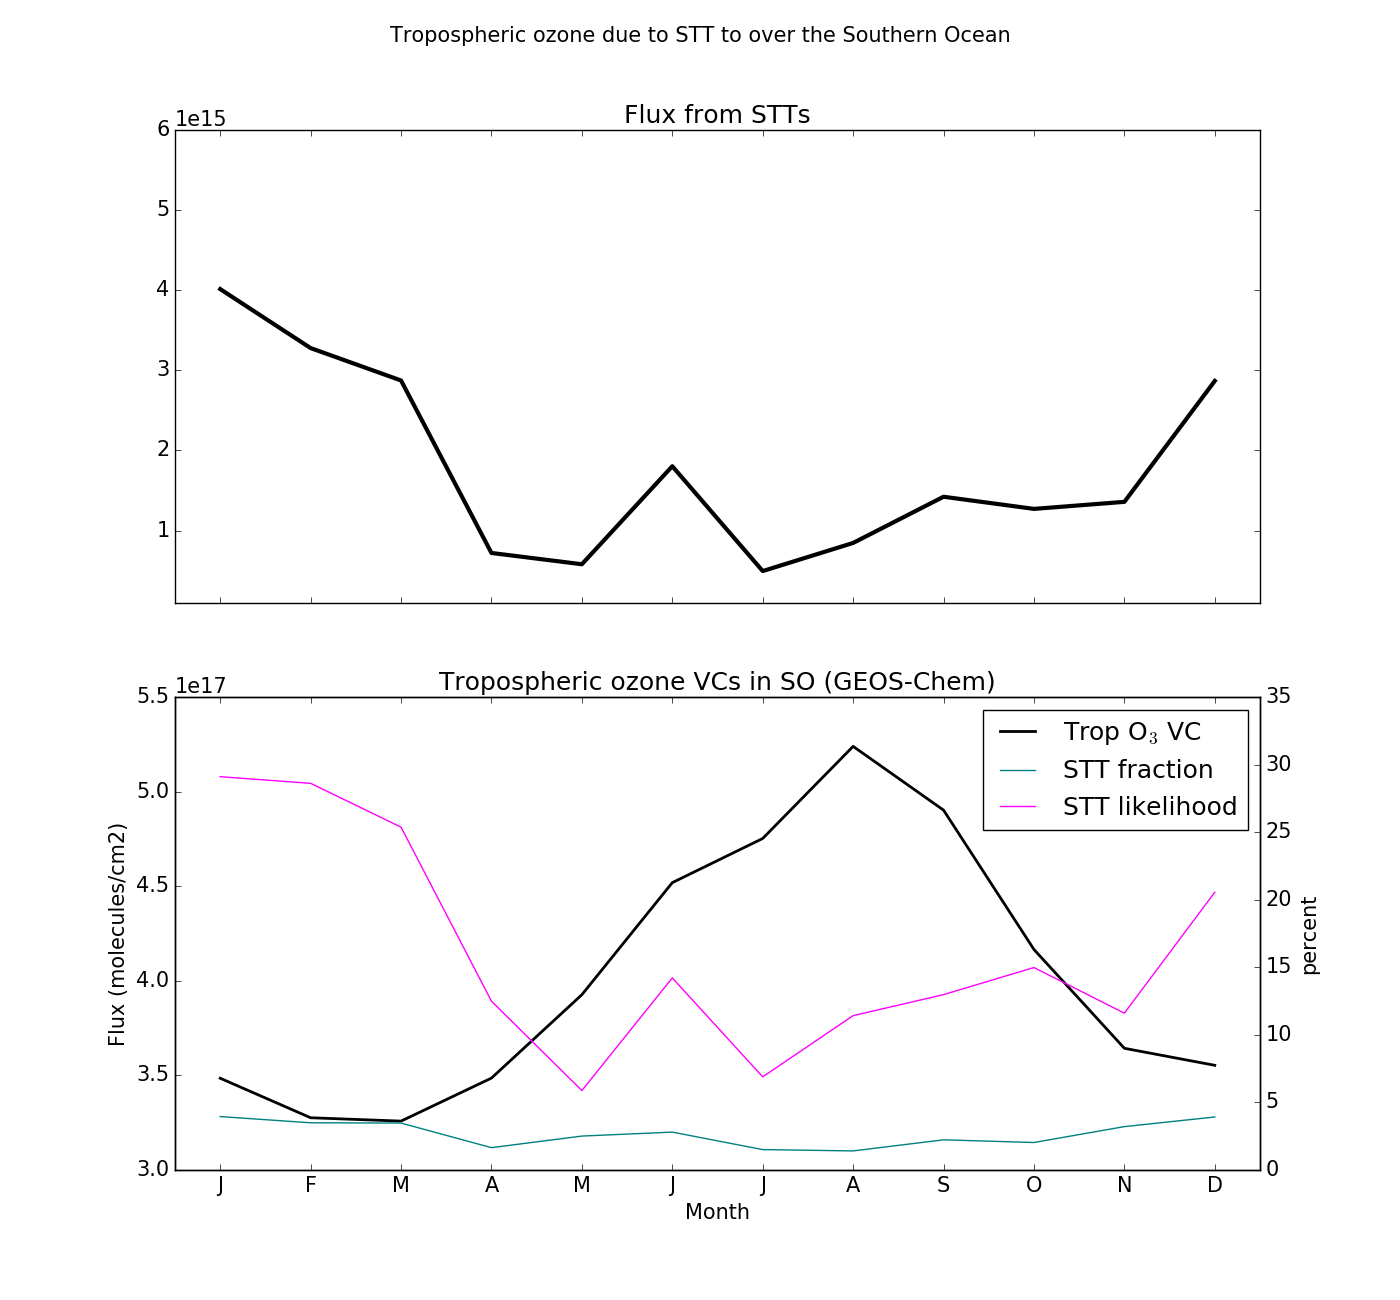
\includegraphics[width=\textwidth]{figures/SO_extrapolation.png}
    \caption{(Top) Estimated contribution of STT to tropospheric ozone columns over the Southern Ocean.
      (Bottom) The three quantities used to calculate (as per the text) the flux estimates shown in the top panel.
      The tropospheric ozone column (left axis) is from GEOS-Chem, while the STT fraction and likelihoods (right axis) are from the ozonesonde measurements.
      The STT fraction is multiplied by 3 to show the seasonality.}
    \label{fig:SOExtrapolation}
  \end{figure}
  
  Our estimate is far less than other estimates of STT flux, due to our conservative estimate of flux within each event, as well as filtering out events which are too close to the tropopause.
  \citet{Olsen2003} use PV and winds from the GEOS reanalysis combined with ozone measurements from the TOMS satellite to estimate that around 210~TG yr$^{-1}$ of ozone flux occurs in 2000 between 30$^{\circ}$S and 60$^{\circ}$S.
  Their estimates show peak ozone flux from winter to early spring (JJAS). 
  At this time of year, we find from the GEOS-Chem simulation the highest overall tropospheric $\Omega_{O3}$, but a relatively low overall STT flux.
  Instead, our results suggest that the STT flux is largest in austral summer (DJFM), primarily due to an increased frequency of STT detections during these months.
  Some legitimate STT events may have been removed due to coincident smoke plumes, which could affect our STT event frequency during winter.
  It is worth noting that the 30$^{\circ}$S to 60$^{\circ}$S latitudes describe the Ferrel cell, while our region of analysis includes some of the Polar cell.
  
  TODO: up to here with Jenny Comments
  
  Global STT flux estimated from an ensemble of models suggests values around 550~Tg yr$^{-1}$ \citep{Stevenson2006}.
  Our estimate of 1.82 is $\sim$0.32~\% of this value, .
  The net flux is also important, although the algorithm used here only examines flux in the downward direction.
  Global net flux (transport from the stratosphere to the troposphere minus opposite transport) is estimated to be 75~Tg yr$^{-1}$ \citep{Sprenger2003}.
  
  Considering the individual event contributions, \citet{Terao2008} estimate much higher STT impacts; where 30--40\% of the tropospheric column is due to STT. 
  Although this figure is based on the Northern Hemisphere during the seasonal STT peak.
  This shows the order of difference between STT flux at various latitudes
  
  
\section{Conclusions}
  
  Ozonesonde data in the Southern Hemisphere provides a satellite-independant quantification of STT ozone transport.
  The frequency and amount of ozone descending from the stratosphere into the troposphere can be estimated from the long time series of tropospheric ozone profiles.
  Using almost ten years of ozonesonde profiles over the southern high latitudes, a clear summer peak is seen for STT occurences at both 38$^{\circ}$S and 55$^{\circ}$S, although not at 69$^{\circ}$S.
  
  We use a Fourier bandpass filter to determine STT ozone transport events.
  The filter removes seasonal tropospheric ozone influences and allows clear detection of ozone-enhanced tongues of air in the troposphere.
  By setting empirical checks, ozonesonde vertical profiles can clearly show tropospheric ozone enhancement which is separated from the stratosphere.
  The cause of these ozone enhancements is examined through the use of satellite and reanalysis datasets on case studies above Melbourne.
  The major causes of STT events found over Melbourne are turbulent weather in the upper troposphere due to low pressure fronts and cut-off low pressure systems.
  TODO: Discuss Davis,Macq here
  
  Integration of the ozone enhancement along the altitude of the ozone profile allows a rough estimate of stratospheric transport for each event.
  Events typically cause a 3\% enhancement of the tropospheric ozone column.
  Within a year this ranges from $1$ to $6 \times 10^{15}$ molecules cm$^{-2}$ ozone enhancement over the southern high latitudes caused by STTs.
  
  GEOS-Chem performs fairly well when compared to ozonesondes at our three sites, with vertical profile averages and seasonal cycles of tropospheric ozone conforming to within $\sim 10$\% (TODO: update when model finishes) of the data, even though the model is looking at the average over 2$^{\circ}$ latitude by 2.5$^{\circ}$ longitude grid boxes.
  
% This bibliography is created by Mendeley
\bibliography{bibliography/Ozone.bib}

\end{document}

